\documentclass{article}

%%%%%%%%%%%%%%%%%%%%%%%%%%%%%%%%%%%%%%%%%%%%
% Packages
%%%%%%%%%%%%%%%%%%%%%%%%%%%%%%%%%%%%%%%%%%%%
\usepackage{amsmath}
\usepackage{amssymb}
\usepackage{tikz}
\usepackage{graphicx}
\usepackage{fancyhdr} % Customize header and footer
\usepackage{listings} % Allows syntax highlighting
\usepackage{lstautogobble}
\usepackage[hidelinks]{hyperref}
\usepackage{float}
\usepackage{subcaption}
\usepackage{pdfpages}
\usepackage[margin=1.0in]{geometry}
\usepackage[backend=biber,style=ieee]{biblatex}
\addbibresource{bibliography.bib}

%%%%%%%%%%%%%%%%%%%%%%%%%%%%%%%%%%%%%%%%%%%%
% General document setup
%%%%%%%%%%%%%%%%%%%%%%%%%%%%%%%%%%%%%%%%%%%%
\usetikzlibrary{positioning}
\setlength{\parindent}{0em}
\graphicspath{ {./images} }

\newcommand{\course}{MEng Project}
\newcommand{\assignment}{\course{} Report}
\newcommand{\name}{Shay Osler}
\newcommand{\clut}{{(0)}}
\newcommand{\tgt}{{(1)}}
\newcommand{\clutj}{{(j,0)}}
\newcommand{\tgtj}{{(j,1)}}
\newcommand{\cluti}{{(i,0)}}
\newcommand{\tgti}{{(i,1)}}
\newcommand{\lcphd}{$\lambda$-CPHD}
\newcommand{\lpdcphd}{$\lambda$-$p_D$-CPHD}

% PDF specific setup, links, title, bookmarks
\hypersetup
{
  colorlinks=true,
  linkcolor=black,
  citecolor=black,
  bookmarks=true,
  pdftitle=\name{} - \assignment{},
  urlcolor=blue
}

% Define formatting for code
\lstset
{
  language=Matlab,
  basicstyle=\ttfamily,
  breaklines=false,
  autogobble=true,
  keywordstyle=\color{blue},
  commentstyle=\color{green}
}

% title
\title{Comparison of Random Finite Set Filters for Multi-Object Tracking}
\author{\name}

% Header and Footer
\pagestyle{fancy}
\lhead{\name}
\chead{}
\rhead{\assignment}

\lfoot{}
\cfoot{\thepage}
\rfoot{}

% Disable numbers on sections, but keep them in table of contents
\setcounter{secnumdepth}{0}

%%%%%%%%%%%%%%%%%%%%%%%%%%%%%%%%%%%%%%%%%%%%
% Content
%%%%%%%%%%%%%%%%%%%%%%%%%%%%%%%%%%%%%%%%%%%%
\begin{document}
\maketitle
\pagebreak


\section*{Preface}
The Gaussian mixture PHD filter and some of the pruning/merging code used in the GMPHD, \lcphd and \lpdcphd were developed as part of the final project for Fall 2022 MAE6760 course. The Labeled Multi Bernoulli (LMB) filter implementation was from a reference implementation sourced from \cite{vo_rfs}.

\section*{Abstract}
Random finite sets present a compelling framework with which to attempt to solve multi-object tracking problems, providing an alternative to other modern Bayesian multi-object tracking methodologies such as joint probabilistic data association or multi-hypothesis tracking. Implementations of a number of different random finite set based filters are compared under simulated multi-object tracking situations with the goals of better understanding the effects of the major filter tuning parameters, and of identifying filter(s) that might be suitable candidates for future tests and application to real world target tracking problems.

\tableofcontents
\listoffigures
\listoftables

\subsection*{List of Symbols}
\begin{table}[h]
  \begin{center}
    \begin{tabular}{ c l }
      $\square^\clut$ & A symbol pertaining to clutter\\
      $\square^\tgt$ & A symbol pertaining to targets\\
      $\square_k$ & A symbol containing values for time $k$\\
      $\langle a, b \rangle$ & Inner product of $a$ and $b$ \\
      $\mathcal{N}(\mu, \Sigma)$ & Gaussian distribution with mean $\mu$ and covariance $\Sigma$\\
      $\beta(a, b)$ & A beta distribution with parameters $a$ and $b$ \\
      $B(a, b)$ & Beta function calculated on $a$ and $b$ \\
      $F$ & Linear state transition matrix, $x_{k+1} = Fx_k$ \\
      $Q$ & Process noise covariance \\
      $H$ & Measurement model \\
      $R$ & Measurement noise \\
      $v$ & The intensity of a random finite set \\
      $J$ & The number of components in an RFS intensity \\
      $p_{D}$ & Probability that an object (clutter or target) is detected\\
      $p_{S}$ & Probability that an object (clutter or target) survives from time $k-1$ to $k$\\
      $\Gamma$ & RFS representing a birth model\\
      $\gamma$ & Intensity of $\Gamma$ \\
      $N_{\Gamma}$ & Mean number of births \\
      $w$ & Component weight \\
      $m$ & Mean of a Gaussian component \\
      $P$ & Covariance of a Gaussian component \\
      $\lambda$ & Clutter rate \\
      $T$ & Truncation threshold for pruning intensities\\
      $U$ & Distance threshold for merging components in an intensity \\
      $J_{max}$& Maximum number of allowed components in an intensity \\
      $N$ & Cardinality of a random finite set \\
      $\ddot{\rho}$ & Cardinality distribution for a random finite set \\
      $Z$ & Set of measurements \\
      $|Z|$ & Cardinality of Z \\
      %\hline
    \end{tabular}
  \end{center}
  \caption{\label{tab:variables}List of symbols}
\end{table}

\section{Introduction}

\section{Algorithms}
GMPHD filter\cite{gmphd}

For this project I implemented ??? RFS based filtering algorithms. The first two filters I implemented were variants of the Cardinalized Probability Hypothesis Density (CPHD) filter. CPHD filters are similar to PHD filters, but whereas the PHD filter only propagates the posterior intensity distribution of the RFS representing the set of tracked targets, the CPHD filter jointly propagates both the posterior intensity distribution and the posterior cardinality distribution.

\subsection{CPHD With Unknown Clutter Rate}
The CPHD filter with unknown clutter rate ($\lambda$-CPHD) proposed in \cite{cphd} attempts to simultaneously estimate the states of tracked targets and the rate of clutter detections (i.e. the expected number of lutter detections at a given time). To do this it models clutter as the returns from a set of ``clutter generator'' objects which could be located at any arbitrary location, and then jointly estimates the positions of the target objects, the cardinality of the target RFS, and the cardinality of the clutter generator RFS. \\
\\
Where necessary throughout this algorithm, symbols pertaining to the clutter RFS are denoted with a superscript $^{(0)}$, and symbols pertaining to the target RFS are denoted with a superscript $^{(1)}$. Subscripts $_{k-1}$, $_k$, and $_{k+1}$ are used to denote symbols pertaining to the previous, current, or next time step respectively. A subscript $_{k|k-1}$ denotes a prediction of a value at time $k$ given the value at time $k-1$.
\\
The intensity of the random finite set representing the targets at time $k$, $v^{(1)}_k$, is modeled as a Gaussian mixture
\begin{equation}
  \label{eq:vk-1}
  v^{(1)}_k = \sum_{i = 1}^{J_k}w_k^i \mathcal{N}(m_k^i,\,P_k^i)
\end{equation}

where $w$, $m$, and $P$ represent the component weights, means, and covariances respectively. The hybrid cardinality distribution representing the total cardinality of targets and clutter generators is given by $\ddot{\rho}$. \\
\\
The dynamics for each target are assumed to be linear with a state transition matrix $F_k$, with additive 0 mean Gaussian noise, with covariance $Q_k$, ie given some state $x_k$
\begin{equation}
  \label{eq:tgt_dynamics}
  x_{k+1} = F_kx_k + \mathcal{N}(0,\,Q_k)
\end{equation}

The detection probabilities for clutter and targets at some time $k$ are given by $p_{Dk}^{(0)}$ and $p_{Dk}^{(1)}$, and likewise the survival probabilities for clutter and targets at time $k$ denoted by $p_{Sk}^{(0)}$ and $p_{Sk}^{(1)}$. The relative likelihood of there being clutter at any location $x$ is represented by $\kappa(x)$, which should be chosen such that the integral over all $x$ (e.g. over the whole field of view) is $1$.\\
\\
The clutter generator birth model is denoted $\Gamma^{(0)}$; however, since the clutter returns themselves are considered independent of the actual state of the clutter generators it is sufficient to only consider the mean number of clutter generator births, $N_{\Gamma k}^{(0)}$. The target birth model is $\Gamma^{(1)}_k$, with intensity $\gamma^{(1)}_k$
\begin{equation}
  \label{eq:tgt_birth}
\gamma^{(1)}_k = \sum_{i=1}^{J_{\gamma k}^{(1)}}w_{\gamma k}^i \mathcal{N}(m_{\gamma k}^i,\,P_{\gamma k}^i)
\end{equation}

and the cardinality distribution of the total number of births, $\ddot{\rho}_{\Gamma k}$, is modelled as a Poisson distribution with parameter $\lambda_\Gamma$ given by
\begin{equation}
  \label{eq:rho_gamma}
\lambda_{\Gamma k} = N_{\Gamma k}^{(0)} + \sum_{i=1}^{J_{\gamma k}^{(1)}}w_{\gamma k}^i 
\end{equation}

\subsubsection{Prediction}
If at time $k-1$ the posterior total cardinality distribution is $\ddot{\rho_{k-1}}$, the posterior mean number of clutter generators is $N^{(0)}_{k-1}$, and the posterior target intensity is given by

\begin{equation}
  \label{eq:vk}
  v^{(1)}_{k-1} = \sum_{i = 1}^{J_{k-1}}w_{k-1}^i \mathcal{N}(m_{k-1}^i,\,P_{k-1}^i)
\end{equation}

then the predicted intensity, $v_{k|k-1}$, will be the sum of the target birth model intensity and the intensity calculated by propagating the mean and covariance of each component in the posterior target intensity through the system dynamics, with the weights scaled by the target survival probability, $p_S^{(1)}$
\begin{align}
  \label{eq:v_predict}
  v_{k|k-1} &= p_{Sk}^{(1)}v_{k-1} + \gamma^{(1)}\\
           &= \sum_{j = 1}^{J_k-1} p^\tgt_{Sk}w_{k-1}^j \mathcal{N}(m_{k|k-1}^j,\,P_{k|k-1}^j) + \gamma^{(1)}_k\\
  m_{k|k-1}^j &= F_km_{k-1}^j\\
  P_{k|k-1}^j &= Q_k+F_kP_{k-1}^jF_k^T
\end{align}
The predicted mean number of clutter generators is similarly the predicted number of surviving clutter generators plus the mean number of clutter births
\begin{equation}
  \label{eq:N0_predict}
  N_{k|k-1}^{(0)} = N_{\gamma k}^{(0)} + p_{Sk}^{(0)}N_{k-1}^{(0)}
\end{equation}

Finally the predicted total cardinality distribution is
\begin{equation}
  \label{eq:rho_predict}
 \ddot{\rho}_{k|k-1}(\ddot{n}) = \sum_{j=0}^{\ddot{n}}\ddot{\rho}_{\Gamma k}(\ddot{n} - j) \sum_{l=j}^\infty {l \choose j}\ddot{\rho}_{k-1}(l)(1-\phi)^{l-j}\phi^j
\end{equation}
where $\phi$ represents the proportion of surviving clutter generators and targets
\begin{equation}
  \label{eq:phi}
  \phi = \frac{p_{Sk}^{(1)}\sum_{i=1}^{J_{k|k-1}}w_{k-1}^{(i)} + P_{Sk}^{(0)}N_{k|k-1}^{(0)}}{\sum_{i=1}^{J_{k|k-1}}w_{k|k-1}^{(i)} + N_{k|k-1}^{(0)}}
\end{equation}
\subsubsection{Update}
Given a set of measurements $Z_k = \{z_1,\;z_2,\;...\;z_{Jzk}\}$ with linear measurement model
\begin{align}
  \label{eq:z}
  z_j = Hx_k + n\\
  n\sim \mathcal{N}(0,\,R)
\end{align}

the updated estimates for target intensity, mean number of clutter generators, and total cardinality are

\begin{equation}
  \label{eq:vk}
  v^{(1)}_k = (1-p_{Dk}^\tgt)w_{Mk}v_{k|k-1} + \sum_{z \in Z_k}\sum_{j=1}^{J_{k|k-1}}w_{Dk}(z)\mathcal{N}(m_k^{(j)},P_k^{(j)})
\end{equation}
\begin{equation}
  \label{eq:N0k}
  N_k^{(0)} = N_{k|k-1}^{(0)}\left( (1-p_{Dk}^\clut)w_{Mk} + \sum_{z \in Z_k}\frac{p_{Dk}^{(0)}\kappa(z)}{ p_{Dk}^{(0)}N_{k|k-1}^{(0)}\kappa_k(z) +  p_{Dk}^{(1)}\sum_{i=1}^{J_{k|k-1}}w_{k|k-1}^{(i)}q_k^{(i)}(z)} \right)
\end{equation}
\begin{equation}
  \label{eq:rhok}
  \ddot{\rho}_k(\ddot{n}) =
  \begin{cases}
    0 & \ddot{n} < |Z_k| \\
    \frac{ \ddot{\rho}_{k|k-1}(\ddot{n})\ddot{\Psi}_k^0(\ddot{n})}{\langle \ddot{\rho}_{k|k-1}, \ddot{\Psi}_k^0 \rangle  } & \ddot{n} \ge |Z_k|
  \end{cases}
\end{equation}

where
\begin{equation}
  \label{eq:mk}
  m_k^{(j)}(z) = m_{k|k-1}^{(j)} + K_k^{(j)}(z - Hm_{k|k-1}^{(j)})
\end{equation}

\begin{equation}
  \label{eq:kalman_gain}
  K_k^{(j)} = P_{k|k-1}^jH^T(HP_{k|k-1}^jH^T + R)^{-1}\\
\end{equation}

\begin{equation}
  \label{eq:Pk}
  P_{k|k}^j = (I - K_k^jH)P_{k|k-1}^j(I - K_k^jH)^T + K_k^jRK_k^{j^T}
\end{equation}

\begin{equation}
  \label{eq:wmk}
  w_{Mk} = \frac{\frac{\langle\ddot{\Psi}_k^1,\ddot{\rho}_{k|k-1}\rangle}{\langle\ddot{\Psi}_k^0,\ddot{\rho}_{k|k-1}\rangle}}{\sum_{i=1}^{J_{k-1}}w_{k-1}^{(i)} + N_{k-1}^{(0)}}
\end{equation}
\begin{equation}
  \label{eq:psi}
  \ddot{\Psi}_k^u(\ddot{n}) =
  \begin{cases}
    0 & \ddot{n} < |Z_k| + u \\
   \frac{\ddot{n}!}{(\ddot{n}-|Z_K|-u)!}\Phi_{k|k-1}^{\ddot{n} - |Z_k|-u} & \ddot{n} \ge |Z_k|+u
  \end{cases}
\end{equation}
\begin{equation}
  \label{eq:Phi}
  \Phi_{k|k-1} = 1 - \frac{p_{Dk}^{(1)}\sum_{i=1}^{J_{k-1}}w_{k-1}^{(i)} + P_{Dk}^{(0)}N_{k-1}^{(0)}}{\sum_{i=1}^{J_{k-1}}w_{k-1}^{(i)} + N_{k-1}^{(0)}}
\end{equation}
\begin{equation}
  \label{eq:wD}
  w_{Dk}^{(j)}(z) = \frac{p_{Dk}^{(1)}w_{k|k-1}^{(j)}q_k^{(j)}(z)}{p_{Dk}^{(0)}N_{k|k-1}^{(0)}\kappa_k(z) +  p_{Dk}^{(1)}\sum_{i=1}^{J_{k|k-1}}w_{k|k-1}^{(i)}q_k^{(i)}(z)  }
\end{equation}
\begin{equation}
  \label{eq:qz}
  q_k^{(j)}(z) = \mathcal{N}(z;Hm_{k|k-1}^{(j)}, HP_{k|k-1}^{(j)}H^T + R)
\end{equation}
and $\langle a, b \rangle$ denotes the inner product of $a$ and $b$.

\subsubsection{Pruning and Merging}
During the prediction step the number of components in the target intensity grows by the number of components in the target birth intensity. Then during the update the number of components increases again by a factor of $|Z_k|$. This can quickly cause the number of components representing the target intensity to grow to a prohibitive size, so after each update step the Gaussian mixture forming $v_{k}$ needs to be pruned yielding a new mixture $\tilde{v}_k$. The pruning process is relatively straightforward. First, calculate the total weight of all components in the mixture
\begin{equation}
  \label{eq:wtotal}
  w_{Total} = \sum_j^Jw^j
\end{equation}

Next, establish some threshold $T$ and discard any components with weight less than $T$. Next merge components that are ``close enough''. For two components $i$ and $j$, define a distance metric
\begin{align}
  \label{eq:gauss_dist}
  d = (m^i - m^j)^T(P^i)^{-1}(m^i - m^j)
\end{align}
Then define a threshold $U$, and starting with the highest weighted component find the set, $L$ of all remaining components in $v$ with distance less than $U$ from the component with the highest weight, including that highest weighted component. Merge the components into a new single gaussian component with weight $\tilde{w}$, mean $\tilde{m}$, and covariance $\tilde{P}$
\begin{align}
  \tilde{w} &= \sum_{i \in L}w^i \label{eq:gauss_merge_w}\\
  \tilde{m} &= \frac{1}{\tilde{w}}\sum_{i \in L}w^im^i \label{eq:gauss_merge_m}\\
  \tilde{P} &= \frac{1}{\tilde{w}}\sum_{i \in L}w^i(P^i + (\tilde{m} - m^i)(\tilde{m} - m^i)^T) \label{eq:gauss_merge_P}
\end{align}
Then find the next highest weighted remaining component, and repeat the merge between that component and any other components that are of lesser weight and close enough, until no more merges can be performed. If there are still more than some desired maximum mixture size, $J_{max}$, components then discard all except the $J_{max}$ highest weighted components. Finally, normalize the weights of the remaining components by a factor of
\begin{equation}
  \label{eq:wnorm}
  \frac{w_{Total}}{\tilde{w}_{Total}}
\end{equation}
where
\begin{equation}
  \label{eq:wtild_total}
  \tilde{w}_{Total} = \sum_j^{\tilde{J}}\tilde{w}^j
\end{equation}

to ensure that the total weight of the intensity is unchanged.

\subsubsection{Estimates}
The weight of each component in the target intensity represents the expected number of targets that component represents, so the estimated cardinality of the target set $N_k^{(1)}$ can now be found by summing the weights of all of of the components of the target intensity
\begin{equation}
  \label{eq:N1k}
  N_k^{(1)} = \sum_j^{\tilde{J}_k}\tilde{w}_k^j
\end{equation}
The estimated target states $\hat{X}_k$ can be extracted by selecting the means of the highest weighted components of $\tilde{v}_k$, replicating each component $round(\tilde{w}_K^j)$ times, until there are $round(N_k^{(1)})$ targets in $\hat{X}_k$. The estimated number of clutter generators is given by $N_k^{(0)}$, and the estimated clutter rate is $\hat{\lambda}_k = p_{Dk}^{(0)}N_k^{(0)}$.

\subsection{CPHD With Unknown Clutter Rate and Detection Probability}
The CPHD with unknown clutter rate and detection probability ($\lambda$-$p_D$-CPHD) as proposed in \cite{cphd}, is similar to the $\lambda$-CPHD filter except that it additionally estimates the detection probabilities for clutter and targets, $p_D^{(0)}$ and $p_D^{(1)}$. The notation used when describing this filter is generally the same as that used for the $\lambda$-CPHD, except where noted. The $\lambda$-$p_D$-CPHD by augments the target and clutter state spaces with an extra state defined on $[0, 1]$ representing the detection probability for that target. The target RFS intensity, $v_k^{(1)}$, is represented as a Beta-Gaussian mixture

\begin{equation}
  \label{eq:v1_bm}
  v_k^\tgt = \sum_{j=1}^{J^\tgt _k}w_k^{(j,1)} \beta(s_k^{(j, 1)}, t_k^{(j, 1)})\mathcal{N}(m_k^i,\,P_k^i)
\end{equation}

Since the clutter returns themselves are considered independent of the actual position of the clutter generators it is sufficient to only consider the probability of detection for each clutter generator, so the clutter RFS intensity, $v_k^{(0)}$ is represented with a Beta mixture

\begin{equation}
  \label{eq:v0_bm}
  v_k^\clut = \sum_{j=1}^{J^\clut _k}w_k^{(j, 0)}\beta(s_k^{(j, 0)}, t_k^{(j, 0)})
\end{equation}

where $s$ and $t$ are the parameters for their respective Beta distributions, and $w$, $m$, and $P$ represent the component weights, means, and covariances respectively. The hybrid cardinality distribution representing the total cardinality of targets and clutter generators is given by $\ddot{\rho}$. \\
\\
The dynamics for each target are assumed to be linear with a state transition matrix $F_k$, with additive 0 mean Gaussian noise, with covariance $Q_k$, ie given some state $x_k$
\begin{equation}
  \label{eq:lpd_tgt_dynamics}
  x_{k+1} = F_kx_k + \mathcal{N}(0,\,Q_k)
\end{equation}

The the survival probabilities for clutter and targets at time $k$ denoted by $p_{Sk}^{(0)}$ and $p_{Sk}^{(1)}$. The relative likelihood of there being clutter at any location $x$ is represented by $\kappa(x)$, which should be chosen such that the integral over all $x$ (e.g. over the whole field of view) is $1$. During each prediction step the variance of each Beta distribution in the target intensity is scaled by a factor $k_{\beta}$, which is usually chosen $k_{\beta} > 1$ so that the variance increases during the prediction step.\\
\\
The clutter generator birth model is denoted $\Gamma^{(0)}$, and like the clutter RFS its intensity is a Beta distribution
\begin{equation}
  \label{eq:lpd_clutter_birth}
  v_{\gamma k}^\clut = \sum_{j=1}^{J^\clut _{\gamma k}}w_{\gamma k}^{(j, 0)}\beta(s_{\gamma k}^{(j, 0)}, t_{\gamma k}^{(j, 0)})
\end{equation}

The target birth model is $\Gamma^{(1)}_k$, with intensity $\gamma^{(1)}_k$ modeled with a Beta-Gaussian mixture
\begin{equation}
  \label{eq:lpd_tgt_birth}
    v_{\gamma k}^\tgt = \sum_{j=1}^{J^\tgt _{\gamma k}}w_{\gamma k}^i \beta(s_{\gamma k}^{(j, 1)}, t_{\gamma k}^{(j, 1)})\mathcal{N}(m_{\gamma k}^i,\,P_{\gamma k}^i)
\end{equation}

and the cardinality distribution of the total number of births, $\ddot{\rho}_{\Gamma k}$, is modelled as a Poisson distribution with parameter $\lambda_\Gamma$ given by
\begin{equation}
  \label{eq:lpd_rho_gamma}
\lambda_{\Gamma k} = N_{\Gamma k}^{(0)} + \sum_{i=1}^{J_{\gamma k}^{(1)}}w_{\gamma k}^i 
\end{equation}

\subsubsection{Prediction}

If at time $k-1$ the posterior total cardinality distribution is $\ddot{\rho_{k-1}}$, the posterior clutter generator intensity is \cite{cphd}
\begin{equation}
  \label{eq:lpd_v0k-1}
  v_{k-1}^\clut = \sum_{j=1}^{J^\clut _{k-1}}w_{k-1}^{(j, 0)}\beta(s_{k-1}^{(j, 0)}, t_{k-1}^{(j, 0)})
\end{equation}

and the posterior target intensity is

\begin{equation}
  \label{eq:lpd_v1k-1}
  v_{k-1}^\tgt = \sum_{j=1}^{J^\tgt _{k-1}}w_{k-1}^{(j,1)} \beta(s_{k-1}^{(j, 1)}, t_{k-1}^{(j, 1)})\mathcal{N}(m_{k-1}^i,\,P_{k-1}^i)  
\end{equation}

then the predicted target intensity, $v^\tgt_{k|k-1}$, will be 
\begin{align}
  \label{eq:lpd_v1_predict}
  v_{k|k-1}^\tgt &= p_{Sk}^{(1)}v_{k-1}^\tgt + \gamma^{(1)}\\
           &= \sum_{j = 1}^{J_k-1}p_{Sk}^\tgt w_{k-1}^j \beta(s_{k|k-1}^{(j, 1)}, t_{k|k-1}^{(j, 1)}) \mathcal{N}(m_{k|k-1}^j,\,P_{k|k-1}^j) + \gamma^{(1)}_k\\
\end{align}

i.e. the target birth RFS intensity plus the posterior intensity that has been predicted forward in time by scaling the weights by the target survival probability, $p_{Sk}^\tgt$, by performing a Kalman filter prediction on the Gaussian parts of the components
\begin{align}
  \label{eq:lpd_kf_predict}
  m_{k|k-1}^j &= F_km_{k-1}^j\\
  P_{k|k-1}^j &= Q_k+F_kP_{k-1}^jF_k^T
\end{align}
and by scaling the variance of the Beta part of each component by $k_\beta$
\begin{equation}
  \label{eq:lpd_skk1}
  s_{k|k-1}^\tgtj = \left( \frac{ \mu_{\beta k|k-1 }^\tgtj \left( 1 -  \mu_{\beta k|k-1 }^\tgtj\right) }
    { \left[ \sigma_{\beta k|k-1}^\tgtj \right]^2  } -1 \right)  \mu_{\beta k|k-1 }^\tgtj
\end{equation}
\begin{equation}
  \label{eq:lpd_tkk1}
  t_{k|k-1}^\tgtj = \left( \frac{ \mu_{\beta k|k-1 }^\tgtj(1 -  \mu_{\beta k|k-1 }^\tgtj) }
    { \left[ \sigma_{\beta k|k-1}^\tgtj \right]^2  } -1 \right)  \left( 1 - \mu_{\beta k|k-1 }^\tgtj \right)
\end{equation}
\begin{equation}
  \label{eq:lpd_muk-1}
  \mu_{\beta k|k-1}^\tgtj = \mu_{\beta k-1}^\tgtj = \frac{s_{k-1}^\tgtj}{s_{k-1}^\tgtj + t_{k-1}^\tgtj}
\end{equation}

\begin{equation}
  \label{eq:lpd_sigk-1}
  \left[ \sigma_{\beta k|k-1}^\tgtj \right]^2 =
  k_\beta\left[ \sigma_{\beta k|k-1}^\tgtj \right]^2 =
  \frac{ s_{k-1}^\tgtj t_{k-1}^\tgtj }{ \left( s_{k-1}^\tgtj + t_{k-1}^\tgtj\right) ^2 \left( s_{k-1}^\tgtj + t_{k-1}^\tgtj + 1 \right) }
\end{equation}


The predicted clutter RFS intensity, $v_{k|k-1}^\clut$ is  predicted number of surviving clutter generators plus the clutter birth intensity \cite{cphd}
\begin{equation}
  \label{eq:lpd_v0_predict}
  v_{k|k-1}^\clut = \gamma_k^\clut + p_{Sk}^\clut v_{k-1}^\clut
\end{equation}

Finally the predicted total cardinality distribution is \cite{cphd}
\begin{equation}
  \label{eq:lpd_rho_predict}
 \ddot{\rho}_{k|k-1}(\ddot{n}) = \sum_{j=0}^{\ddot{n}}\ddot{\rho}_{\Gamma k}(\ddot{n} - j) \sum_{l=j}^\infty {l \choose j}\ddot{\rho}_{k-1}(l)(1-\phi)^{l-j}\phi^j
\end{equation}
where $\phi$ represents the proportion of surviving clutter generators and targets
\begin{equation}
  \label{eq:lpd_phi}
  \phi = \frac{p_{Sk}^\tgt\sum_{j=1}^{J_{k-1}^\tgt}w_{k-1}^\tgtj + P_{Sk}^\clut \sum_{j=1}^{J_{k-1}^\clut}w_{k-1}^\clutj}{\sum_{j=1}^{J_{k-1}^\tgt}w_{k-1}^\tgtj + \sum_{j=1}^{J_{k-1}^\clut}w_{k-1}^\clutj}
\end{equation}

\subsubsection{Update}

Given a set of measurements $Z_k = \{z_1,\;z_2,\;...\;z_{Jzk}\}$ with linear measurement model
\begin{align}
  \label{eq:lpd_z}
  z_j = Hx_k + n\\
  n\sim \mathcal{N}(0,\,R)
\end{align}

the updated estimates for target RFS intensity, clutter generator RFS intensity, and total cardinality are \cite{cphd}

\begin{equation}
  \label{eq:lpd_vk}
  \begin{aligned}
    v^\tgt_k = \sum_{j=1}^{J_{k|k-1}^\tgt}w_{Mk}^\tgtj \beta(s_{k|k-1}^{(j, 1)}, t_{k|k-1}^{(j, 1)}+1) \mathcal{N}(m_{k|k-1}k^\tgtj,P_{k|k-1}^\tgtj) \\
    + \sum_{z \in Z_k}\sum_{j=1}^{J_{k|k-1}^\tgt}w_{Dk}^\tgtj(z) \beta(s_{k|k-1}^{(j, 1)}+1, t_{k|k-1}^{(j, 1)})  \mathcal{N}(m_k^{(j)},P_k^{(j)})
  \end{aligned}
\end{equation}

\begin{equation}
  \label{eq:N0k}
  v^\clut_k = \sum_{j=1}^{J_{k|k-1}^\clut}w_{Mk}^\clutj \beta(s_{k|k-1}^\clutj, t_{k|k-1}^\clutj+1)
  + \sum_{z \in Z_k}\sum_{j=1}^{J_{k|k-1}^\clut}w_{Dk}^\clutj(z) \beta(s_{k|k-1}^\clutj+1, t_{k|k-1}^\clutj)  
\end{equation}
  
\begin{equation}
  \label{eq:lpd_rhok}
  \ddot{\rho}_k(\ddot{n}) =
  \begin{cases}
    0 & \ddot{n} < |Z_k| \\
    \frac{ \ddot{\rho}_{k|k-1}(\ddot{n})\ddot{\Psi}_k^0(\ddot{n})}{\langle \ddot{\rho}_{k|k-1}, \ddot{\Psi}_k^0 \rangle  } & \ddot{n} \ge |Z_k|
  \end{cases}
\end{equation}

where
\begin{equation}
  \label{eq:lpd_mk}
  m_k^{(j)}(z) = m_{k|k-1}^{(j)} + K_k^{(j)}(z - Hm_{k|k-1}^{(j)})
\end{equation}

\begin{equation}
  \label{eq:lpd_kalman_gain}
  K_k^{(j)} = P_{k|k-1}^jH^T(HP_{k|k-1}^jH^T + R)^{-1}\\
\end{equation}

\begin{equation}
  \label{eq:lpd_Pk}
  P_{k|k}^j = (I - K_k^jH)P_{k|k-1}^j(I - K_k^jH)^T + K_k^jRK_k^{j^T}
\end{equation}

\begin{equation}
  \label{eq:lpd_psi}
  \ddot{\Psi}_k^u(\ddot{n}) =
  \begin{cases}
    0 & \ddot{n} < |Z_k| + u \\
   \frac{\ddot{n}!}{(\ddot{n}-|Z_K|-u)!}\Phi_{k|k-1}^{\ddot{n} - |Z_k|-u} & \ddot{n} \ge |Z_k|+u
  \end{cases}
\end{equation}
\begin{equation}
  \label{eq:lpd_Phi}
  \Phi_{k|k-1} = 1 - \frac{\sum_{j=1}^{J_{k|k-1}^\tgt}w_{k|k-1}^\tgtj p_{Dk|k-1}^\tgtj + \sum_{j=1}^{J_{k|k-1}^\clut}w_{k|k-1}^\clutj p_{Dk|k-1}^\clutj}
  {\sum_{j=1}^{J_{k|k-1}^\tgt}w_{k|k-1}^\tgtj + \sum_{j=1}^{J_{k|k-1}^\clut}w_{k|k-1}^\clutj}
\end{equation}

\begin{equation}
  \label{eq:pdkk1}
  p_{Dk|k-1}^{(j,u)} = \frac{ s_{k|k-1}^{(j, u)}}{s_{k|k-1}^{(j, u)} + t_{k|k-1}^{(j, u)}},\;u=0,1
\end{equation}

\begin{equation}
  \label{eq:lpd_wmk}
  w_{Mk}^{(j,u)} = \frac{
    \frac{B\left( s_{k|k-1}^{(j,u)},t_{k|k-1}^{(j,u)}+1\right)}{B\left( s_{k|k-1}^{(j,u)},t_{k|k-1}^{(j,u)}\right)}
    \frac{\langle\ddot{\Psi}_k^1,\ddot{\rho}_{k|k-1}\rangle}{\langle\ddot{\Psi}_k^0,\ddot{\rho}_{k|k-1}\rangle}  }
  {\sum_{i=1}^{J_{k-1}^\tgt}w_{k|k-1}^\tgti + \sum_{i=1}^{J_{k-1}^\clut}w_{k|k-1}^\cluti},\; u=0,1
\end{equation}

\begin{equation}
  \label{eq:lpdwD0}
  w_{Dk}^\clutj(z) = \frac{w_{k|k-1}^\clutj  \frac{B\left( s_{k|k-1}^\clutj+1,t_{k|k-1}^\clutj\right)}{B\left( s_{k|k-1}^\clutj,t_{k|k-1}^\clutj\right)}\kappa(z)}
  {\sum_{i=1}^{J_{k|k-1}^\clut}w_{k|k-1}^\cluti p_{Dk|k-1}^\cluti\kappa_k(z) +  \sum_{i=1}^{J_{k|k-1}^\tgt}w_{k|k-1}^\tgti p_{Dk|k-1}^\tgti q_k^{(i)}(z)  }
\end{equation}

\begin{equation}
  \label{eq:lpdwD1}
  w_{Dk}^\tgtj(z) = \frac{w_{k|k-1}^\tgtj  \frac{B\left( s_{k|k-1}^\tgtj+1,t_{k|k-1}^\tgtj\right)}{B\left( s_{k|k-1}^\tgtj,t_{k|k-1}^\tgtj\right)}q_k^{(j)}(z)}
  {\sum_{i=1}^{J_{k|k-1}^\clut}w_{k|k-1}^\cluti p_{Dk|k-1}^\cluti\kappa_k(z) +  \sum_{i=1}^{J_{k|k-1}^\tgt}w_{k|k-1}^\tgti p_{Dk|k-1}^\tgti q_k^{(i)}(z)  }
\end{equation}

\begin{equation}
  \label{eq:qz}
  q_k^{(j)}(z) = \mathcal{N}(z;Hm_{k|k-1}^{(j)}, HP_{k|k-1}^{(j)}H^T + R)
\end{equation}
with $\langle a, b \rangle$ denoting the inner product of $a$ and $b$ and $B(a, b)$ the Beta function.


\subsubsection{Pruning and Merging}
Like the $\lambda$-CPHD filter the number of components in the target and clutter intensities will quickly grow and thus require pruning and merging. Pruning and merging of clutter and target intensities both follow the same general algorithm that was used for the $\lambda$-CPHD. First discard any components with weight less than some minimum $T$. Then, starting with the highest weighted component select all components ``closer'' than some threshold $U$ by some distance metric and merge the components then remove all of the components that were merged and repeat with the highest weighted remaining component. Then if discard the lowest weighted components until there are no more than $J_{max}$ components. Finally, normalize the weights of the remaining components to ensure that the total weight of the mixture is unchanged.\\
\\
For the clutter RFS intensity the distance metric used was the squared Hellinger distance between two Beta distributions
\begin{equation}
  \label{eq:hellinger_beta}
  H^2\left( \beta(s_1,t_1),\beta(s_2,t_2)\right) = 1 - \frac{B\left( \frac{s_1+s_2}{2},\frac{t_1+t_2}{2}\right)}{\sqrt{B(s_1,t_1)B(s_2,t_2)}}
\end{equation}
and a set $L$ of Beta mixture component were merged into a new component $\tilde{\beta}(\tilde{s},\tilde{t})$ with weight $\tilde{w}$ via
\begin{equation}
  \label{eq:beta_merge_w}
  \tilde{w} = \sum_{i \in L}w^i
\end{equation}
\begin{equation}
  \label{eq:beta_merge_s}
  \tilde{s} = \left( \frac{ \tilde{\mu} \left( 1 - \tilde{\mu} \right) }
    { \left[ \tilde{\sigma} \right]^2  } -1 \right)  \tilde{\mu}
\end{equation}

\begin{equation}
  \label{eq:beta_merge_t}
  \tilde{t} = \left( \frac{ \tilde{\mu} \left( 1 - \tilde{\mu} \right) }
    { \left[ \tilde{\sigma} \right]^2  } -1 \right)  \left( 1-\tilde{\mu} \right)
\end{equation}

\begin{equation}
  \label{eq:beta_mu_merge}
  \tilde{\mu} = \frac{ 1 }{\tilde{w}}\sum_{i \in L}w^i\mu^i
\end{equation}

\begin{equation}
  \label{eq:beta_sigsq_merge}
  \left[ \tilde{\sigma} \right]^2 = \frac{ 1 }{\tilde{w}}\sum_{i \in L}w^i\left[ \sigma^i \right]^2
\end{equation}

\begin{equation}
  \label{eq:beta_mu}
  \mu^i = \frac{s^i}{s^i + t^i}
\end{equation}

\begin{equation}
  \label{eq:beta_sigsq}
  \left[ \sigma^i \right]^2 =
  \frac{ s^i t^i }{ \left( s^i + t^i\right) ^2 \left( s^i + t^i + 1 \right) }
\end{equation}
For the target RFS intensity the same distance metric, equation \eqref{eq:gauss_dist}, as for the Gaussian mixtures of the $\lambda$-CPHD filter was used. The Gaussian portions of each component were likewise merged via equations \eqref{eq:gauss_merge_w} - \eqref{eq:gauss_merge_P}, and the Beta portions of each component were merged via equations \eqref{eq:beta_merge_w} - \eqref{eq:beta_sigsq}.

\subsubsection{Estimates}
The estimated cardinalities of the target and clutter random finite sets can be found by summing the weights of all of the components in their respective intensities
\begin{equation}
  \label{eq:lpd_N}
  N_k^{(u)} = \sum_j^{\tilde{J}^{(u)}}\tilde{w}^{(u)}_j,\;u=0,1
\end{equation}
The detection probability for each component is the mean of the Beta distribution associated with that component
\begin{equation}
  \label{eq:pdk}
  p_{Dk}^{(j,u)} = \frac{ \tilde{s}_{k}^{(j, u)}}{\tilde{s}_{k}^{(j, u)} + \tilde{t}_{k}^{(j, u)}},\;u=0,1
\end{equation}
and estimated clutter rate is
\begin{equation}
  \label{eq:lpd_lambda_hat}
  \hat{\lambda}_k = \sum_j^{\tilde{J}_k^\clut}\tilde{w}^\clut_jp_{Dk}^\clutj 
\end{equation}
The target position estimates, $\hat{X}_k$, can be found as for the $\lambda$-CPHD by selecting the means of the highest weighted components of $\tilde{v}_k$, replicating each component $round(\tilde{w}_K^\tgtj)$ times, until there are $round(N_k^\tgt)$ targets in $\hat{X}_k$.

\subsection{Adaptive Labeled Multi Bernoulli Filter}
An adaptive labeled multi-Bernoulli (LMB) filter was implemented by combining a (slightly) modified Labeled Multi Bernoulli\cite{lmb} filter with the $\lambda$-$p_D$-CPHD filter described above, using the same architecture that \cite{adaptive_dglmb} used to make an adaptive $\delta$-generalized labeled multi Bernoulli filter. An adaptive labeled multi-Bernoulli filter was chosen over an adaptive $\delta$-generalized labeled multi Bernoulli filter because \cite{lmb} showed that the LMB filter offers performance that is almost as good as the $\delta$-generalized labeled multi Bernoulli filter, but with a significantly lower computational cost.

\section{Results}
Numerical studies were done to assess the performance of the filters at tracking objects under varying conditions (e.g.\ clutter rate, detection probability) and with varying parameters. The system simulation and filters were run in Matlab. 10 moving targets were simulated moving through the field of view of a simulated sensor. The targets were simulated with a linear constant velocity model with additive Gaussian noise. The simulation time step was set to $1$ for simplicity.

\begin{align}
  x_{k+1} &= Fx_k + \mathcal{N}(0, Q)\\
  F &=
  \begin{bmatrix}
    1 & 0 & 1 & 0\\
    0 & 1 & 0 & 1\\
    0 & 0 & 1 & 0\\
    0 & 0 & 0 & 1
  \end{bmatrix}\;\;
                Q
                = \sigma^2_v
  \begin{bmatrix}
    \frac{1}{4} & 0 & \frac{1}{2} & 0\\
    0 & \frac{1}{4} & 0 & \frac{1}{2}\\
     \frac{1}{2} & 0 & 1 & 0\\
    0 &  \frac{1}{2} & 0 & 1
  \end{bmatrix}\\           
\end{align}

The simulated sensor was a (very) rough approximation of a forward looking sonar with a range of 40m, and a field of view of 90 degrees.\\
\\
The targets were each ``born'' at a random time step during the first 20\% of the simulation duration. Each target was initialized at randomly chosen location within the center 45 degrees of the sonar field of view, at a range between 10m and 20m. The targets were initialized with a random direction of travel with an initial velocity of .25m/s.\\
\\
At each time step a measurement was generated for each target that was within the field of view with probability $p_D = 0.9$. The measurements consisted of the target position corrupted by 0 mean Gaussian noise with covariance
\begin{equation}
  \label{eq:R_true}
  R =
  \begin{bmatrix}
    .25 & 0\\
    0 & .75 \\
  \end{bmatrix}
\end{equation}

Additionally, some number of clutter returns with locations sampled from a uniform distribution over the field of view were returned. The number of clutter returns on any given time step was a random number sampled from a Poisson distribution with parameter $\lambda = 10$, so on average each measurement would have an equal number of clutter and target returns. 10 simulation runs of 100 time steps each was run for each simulator.\\

\begin{figure}[H]
  \centering
  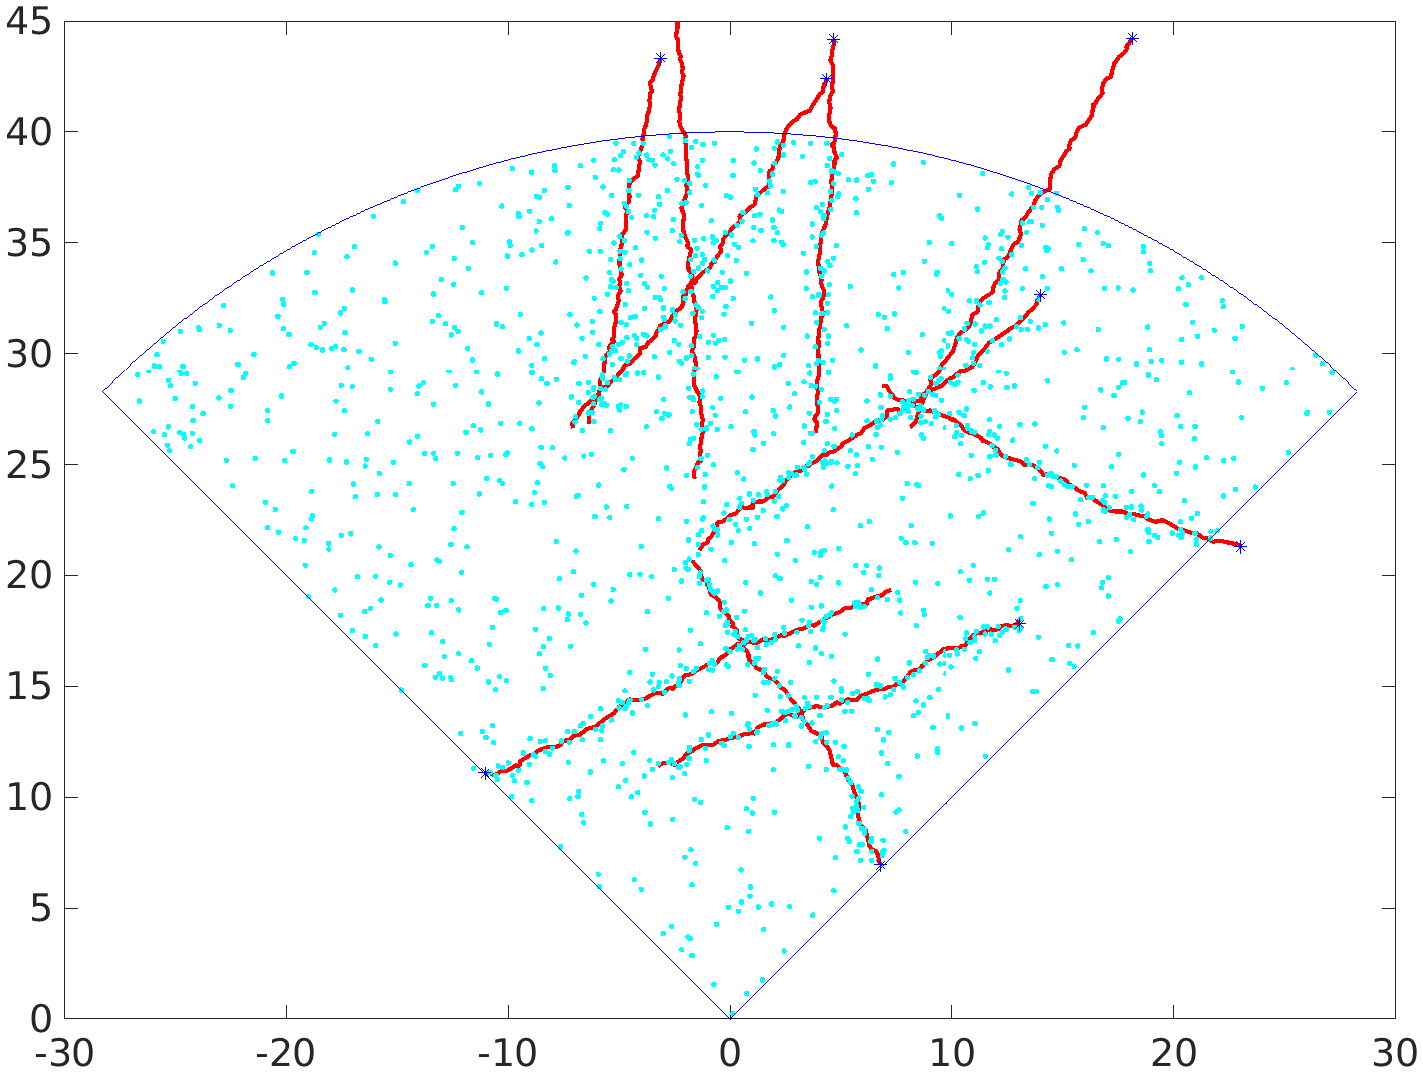
\includegraphics[width=.75\linewidth]{track_obs.png}
  \label{fig:track_obs}
  \caption{Target Tracks (red) and measurements (cyan) from 100 time steps}
\end{figure}

For all of the tests all filters were configured as follows unless noted otherwise. Parameters were chosen to match the analogous true system system parameter. The clutter likelihood $\kappa$ was set to be uniform across the field of view, $\kappa = 1/A_{FOV}$ where $A_{FOV} = \pi * 40^2/4$ is the area of the field of view. The target birth model intensity was a single Gaussian component covering the expected birth area with
\begin{equation}
  \label{eq:target_birth_model}
  \mu =
  \begin{bmatrix}
    20 \\
    0
  \end{bmatrix},\;\;
  \Sigma =
  \begin{bmatrix}
    40 & 0 \\
    0 & 80
  \end{bmatrix}
\end{equation}

\begin{figure}[H]
  \centering
  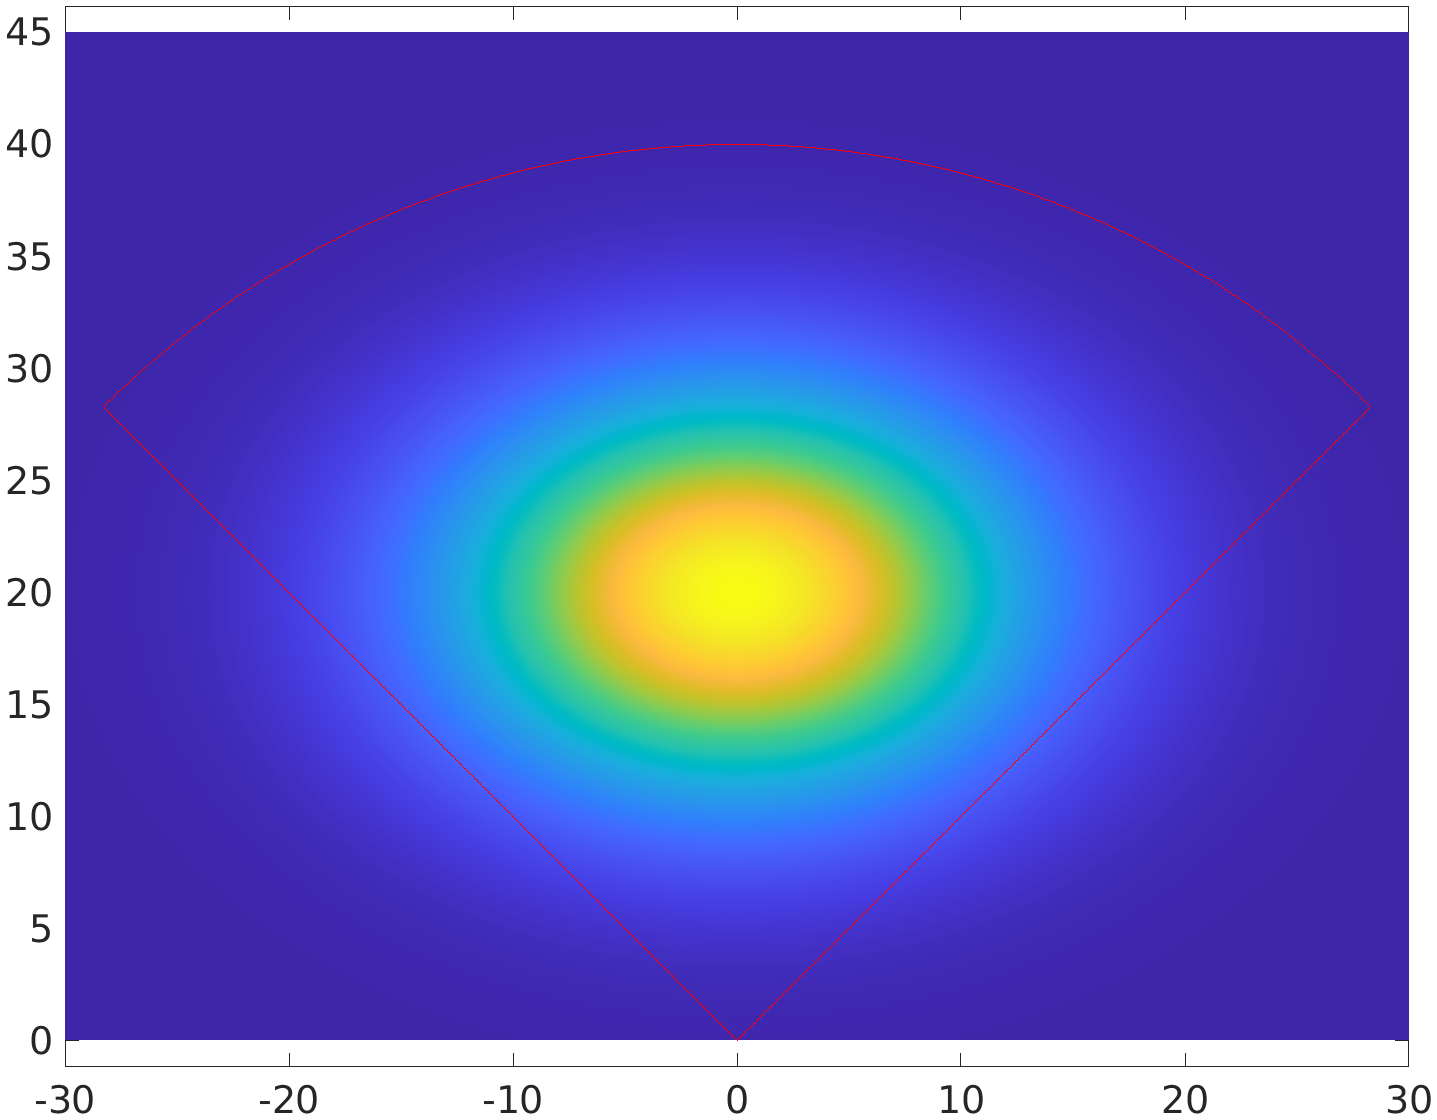
\includegraphics[width=.75\linewidth]{bm2.png}
  \label{fig:birth_model}
  \caption{Birth model}
\end{figure}
and a weight of $N_\Gamma^\tgt = .01$. The target and clutter survival probabilities were set to $p_S^\clut = p_S^\tgt = .9$ For pruning and merging the target intensity the minimum weight was $T = 1e-5$, the merging distance was set to $U = 4$, and the maximum number of components to keep was set to $J_{max} = 100$. The initial cardinality distribution was set to a uniform distribution on the range $[0, 100]$. For the $\lambda$-CPHD filter the clutter birth model $N_\Gamma^\clut$ was set to $5$, and the clutter detection probability $p_D^\clut$ was set to $0.2$. For the $\lambda$-$p_D$-CPHD filter the clutter birth model intensity was a single beta distribution component with $s=1$, $t=1$ and weight $N_\Gamma^\clut = 5$. The beta distribution dilation factor $k_\beta$ was set to $1.5$. For pruning and merging the clutter intensity the the minimum weight was $T = 1e-5$, the merging distance was set to $U = .03$, and the maximum number of components to keep was set to $J_{max} = 100$. For the LMB and adaptive LMB filters the maximum number of tracks was set to 100, the number of update components was set to 1000, and the maxium number of components per track was set to 10. \\

Performance was assessed primarily with the optimal subpattern assignment (OSPA)\cite{OSPA} distance. The OSPA distance is a metric designed to measure the performance of a multi-object tracking algorithm. The OSPA distance seeks to meaningfully capture both cardinality and tracking errors, and the overall OSPA distance as well as the location and cardinality components are reported for each test. The OSPA metrics were calculated with the order set to $1$ and  a cutoff distance of $10$.

\subsection{Optimal Filters}
The first test compared the performance of ``optimal'' filters, configured as described above with as many parameter as possible exactly matching the simulated system.
\begin{figure}[h]
  \centering
  \begin{subfigure}[t]{0.32\textwidth}
    \centering
    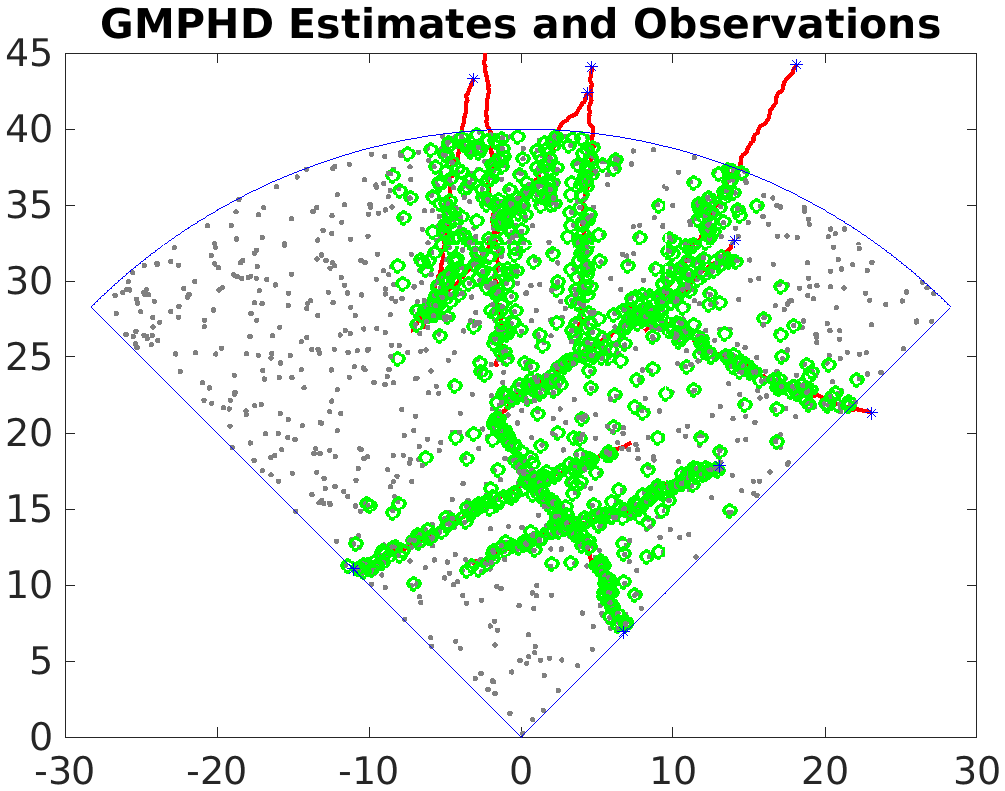
\includegraphics[width=1\linewidth]{gmphd_tracks.png}
    %\caption{Lorem ipsum}
  \end{subfigure}%
  ~ 
  \begin{subfigure}[t]{0.32\textwidth}
    \centering
    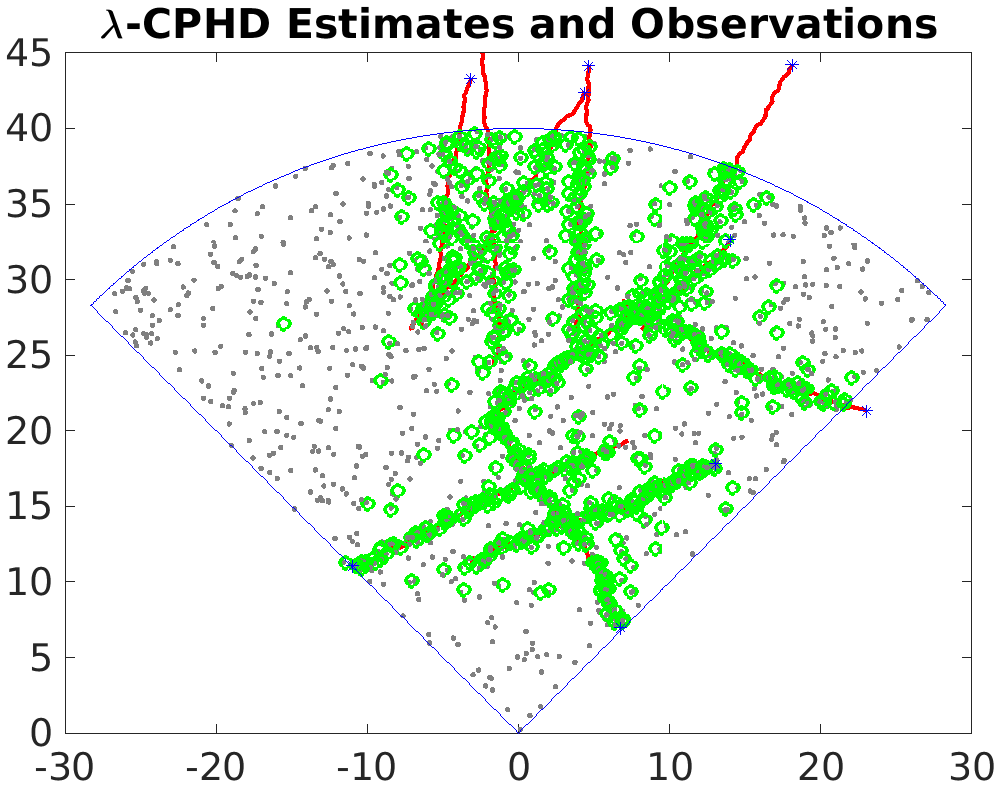
\includegraphics[width=1\linewidth]{lcphd_tracks.png}
    %\caption{Lorem ipsum}
  \end{subfigure}
  ~
  \begin{subfigure}[t]{0.32\textwidth}
    \centering
    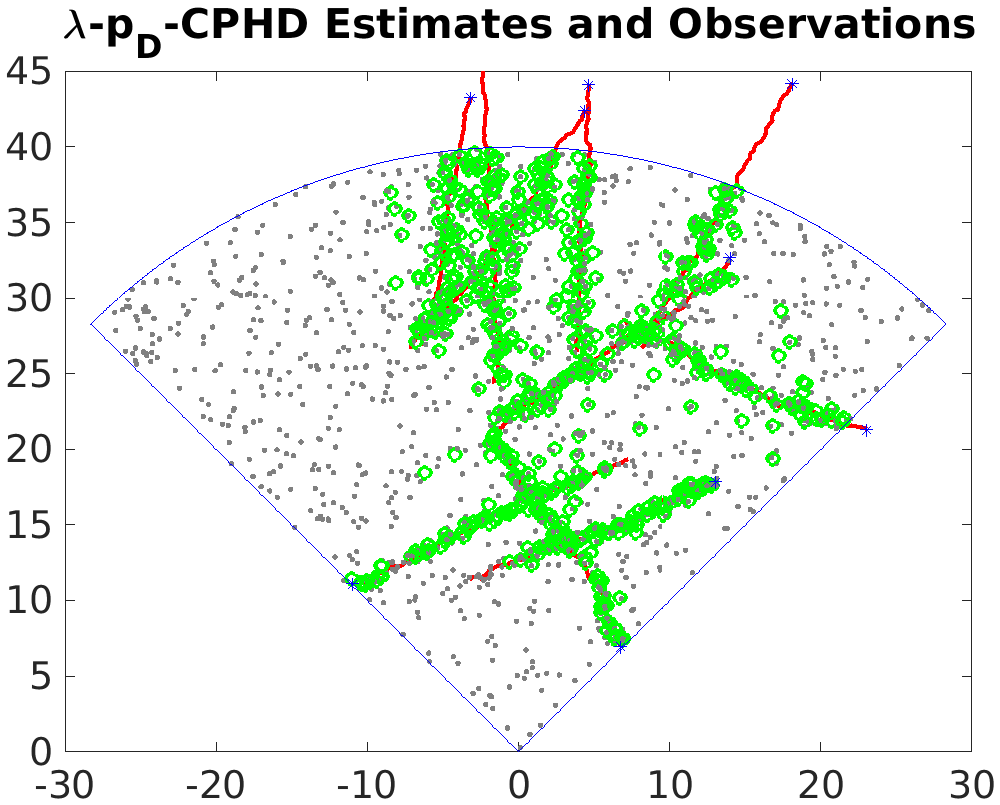
\includegraphics[width=1\linewidth]{lpdcphd_tracks.png}
    %\caption{Lorem ipsum}
  \end{subfigure}%
\\ \medskip
    \begin{subfigure}[t]{0.32\textwidth}
    \centering
    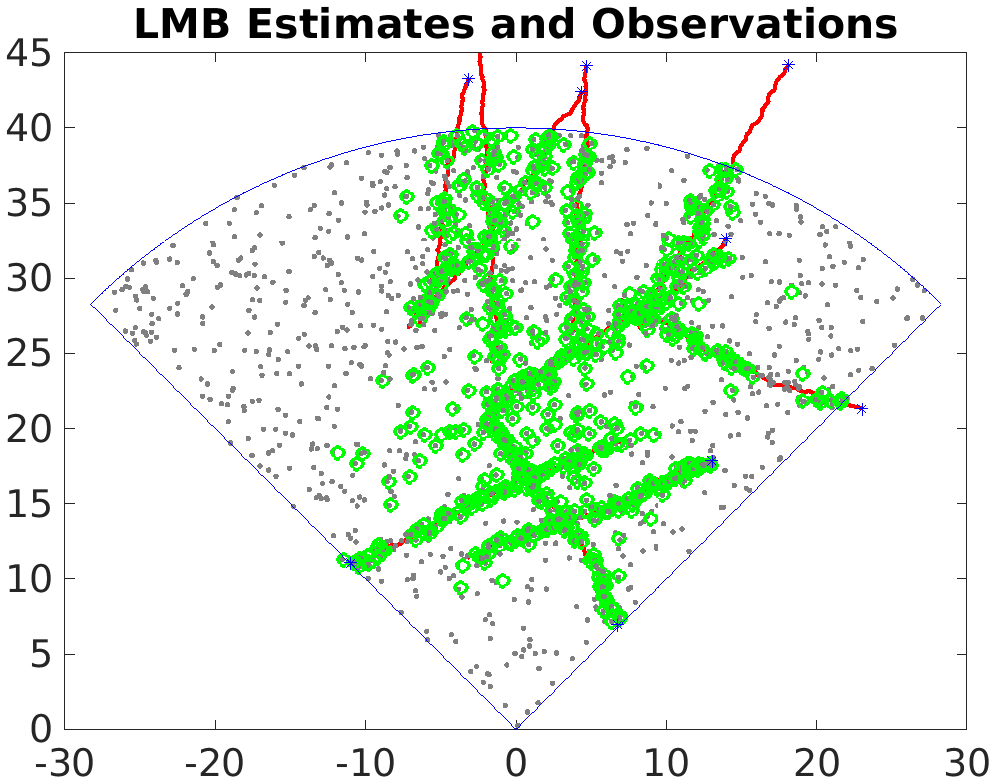
\includegraphics[width=1\linewidth]{lmb_tracks.png}
    %\caption{Lorem ipsum}
  \end{subfigure}%
  ~ 
  \begin{subfigure}[t]{0.32\textwidth}
    \centering
    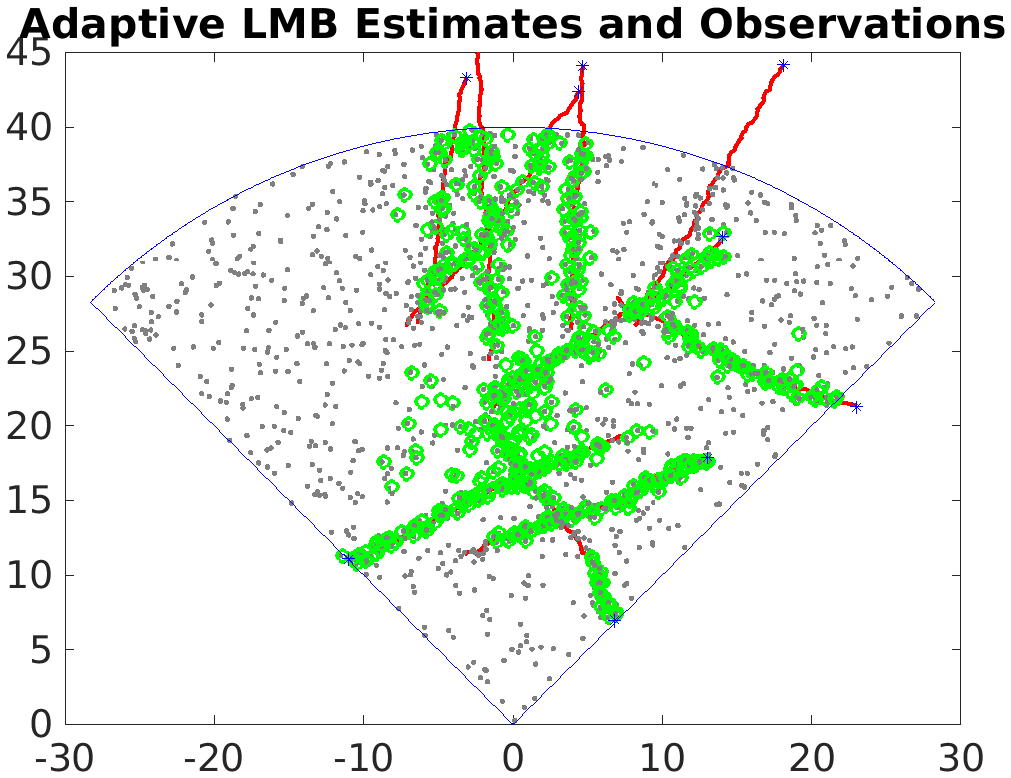
\includegraphics[width=1\linewidth]{almb_tracks.png}
    %\caption{Lorem ipsum}
  \end{subfigure}
  \caption{Example actual target tracks (red), measurements (grey), and target position estimates (green) from one simulation run with optimal parameters.}
\end{figure}

\begin{table}[H]
  \centering
  \begin{tabular}{ c | c| c| c| c| c| c }
    & RMS $N_{err}$ & Mean $N_{err}$ & Std $N_{err}$ & Mean OSPA & Mean OSPA Loc. & Mean OSPA Card.\\
    \hline
    $GMPHD$ & 1.63 & -0.163 & 1.63 & 3.16 & 0.871 & 2.39 \\ 
    $\lambda-CPHD$ & 1.66 & -0.597 & 1.55 & 2.78 & 1.21 & 1.67 \\ 
    $\lambda-p_D-CPHD$ & 2.04 & 1.08 & 1.74 & 3.35 & 0.976 & 2.47 \\ 
    $LMB$ & 1.08 & -0.0168 & 1.08 & 2.47 & 1.47 & 1.1 \\ 
    $Adaptive LMB$ & 2.3 & 1.23 & 1.95 & 3.32 & 1.26 & 2.15 \\ 
  \end{tabular}
  \caption{Performance of optimal filters}
  \label{tab:optimal}
\end{table}
These results generally align with the expected relative performance of the different filters. The LMB filter, with a mean cardinality error of only -.017 has the best performance. The extremely low cardinality error aligns with the theoretical expectations that the filter produce an uniased cardinality estimate under optimal conditions. The GMPHD filter and the $\lambda$-CPHD filter trail the LMB filter in OSPA and cardinality performance. Finally, the two worst performing filters are the $\lambda$-$p_D$-CPHD and the adaptive LMB filter. This is expected under these circumstances because these filters must estimate parameters that the other filters have been provided the true value for. Qualitatively all of the filters appear to be able to provide reasonable cardinality and tracking estimates under these optimal conditions.
\begin{figure}[H]
  \centering
  \begin{subfigure}[t]{0.49\textwidth}
    \centering
    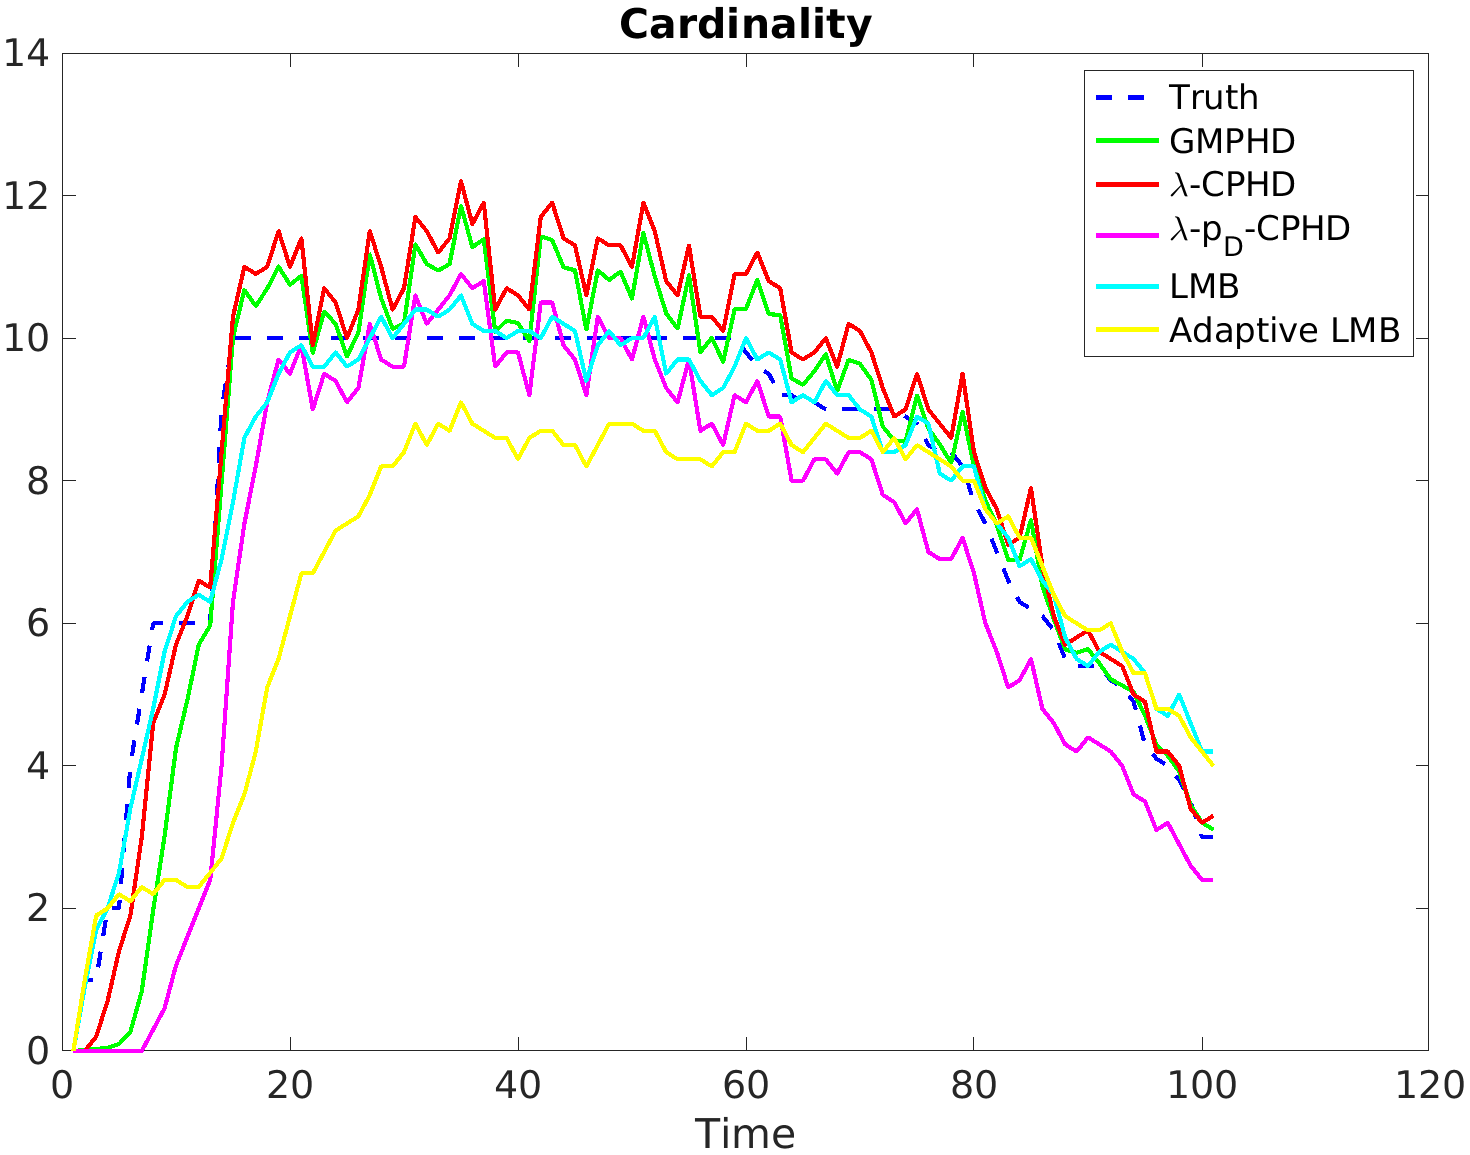
\includegraphics[width=1\linewidth]{optimal/cardinality.png}
    \caption{Cardinality estimates}
  \end{subfigure}%
  ~ 
  \begin{subfigure}[t]{0.49\textwidth}
    \centering
    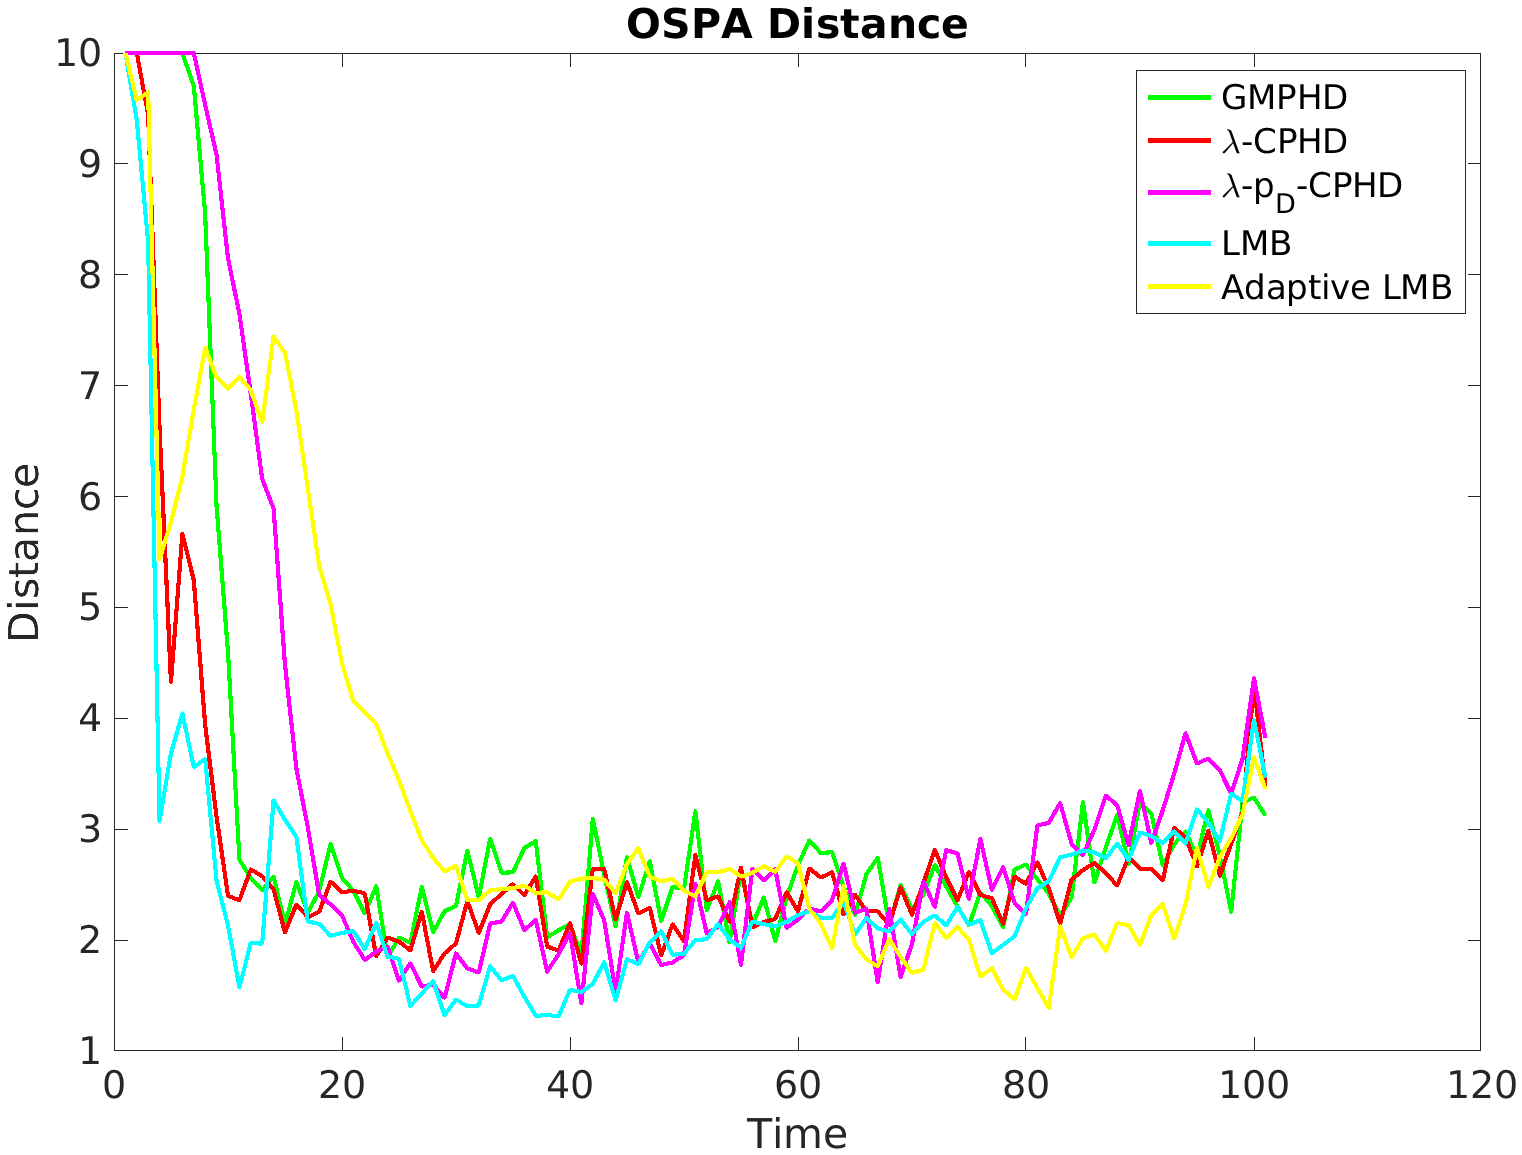
\includegraphics[width=1\linewidth]{optimal/ospa.png}
    \caption{OSPA distances}
  \end{subfigure}
\caption{Cardinality estimates and OSPA distances for optimal estimators}
\end{figure}

\begin{figure}[H]
  \centering
  \begin{subfigure}[t]{0.32\textwidth}
    \centering
    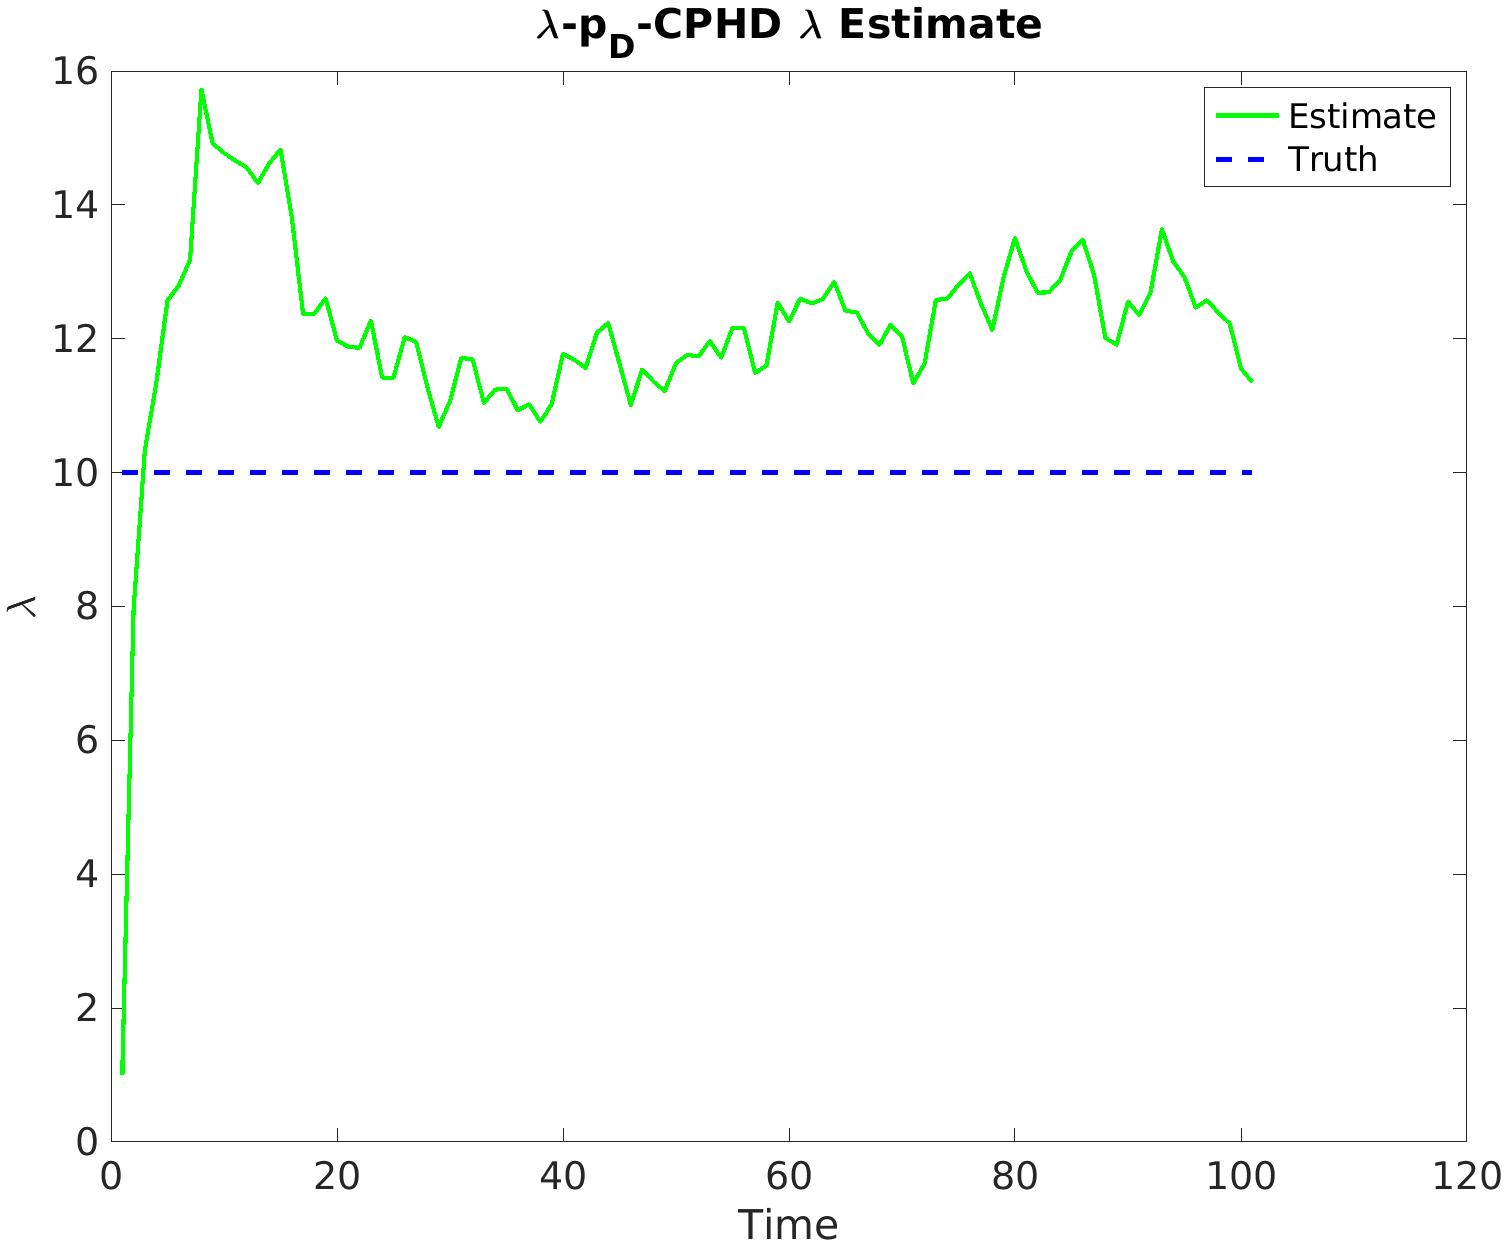
\includegraphics[width=1\linewidth]{optimal/lpdcphd_lambda_hat.png}
    \caption{Clutter rate}
  \end{subfigure}%
  ~ 
  \begin{subfigure}[t]{0.32\textwidth}
    \centering
    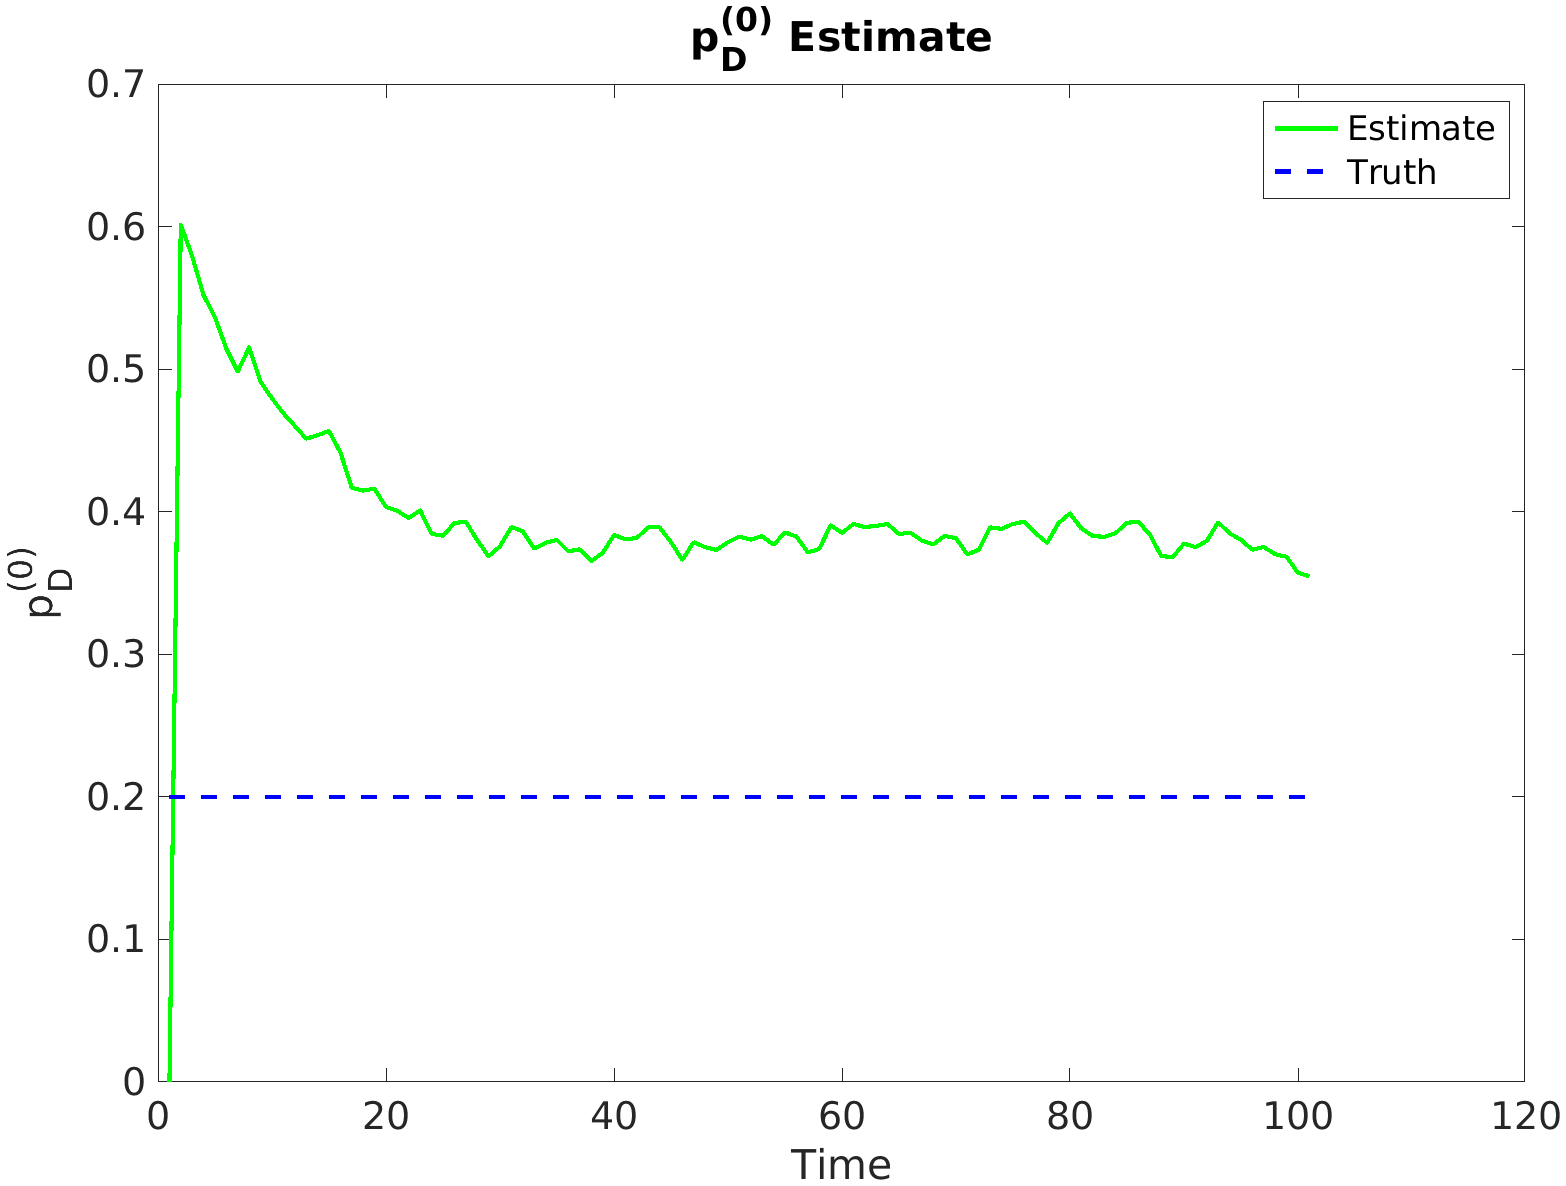
\includegraphics[width=1\linewidth]{optimal/pd0_hat.png}
    \caption{Clutter detection probability}
  \end{subfigure}
  ~ 
  \begin{subfigure}[t]{0.32\textwidth}
    \centering
    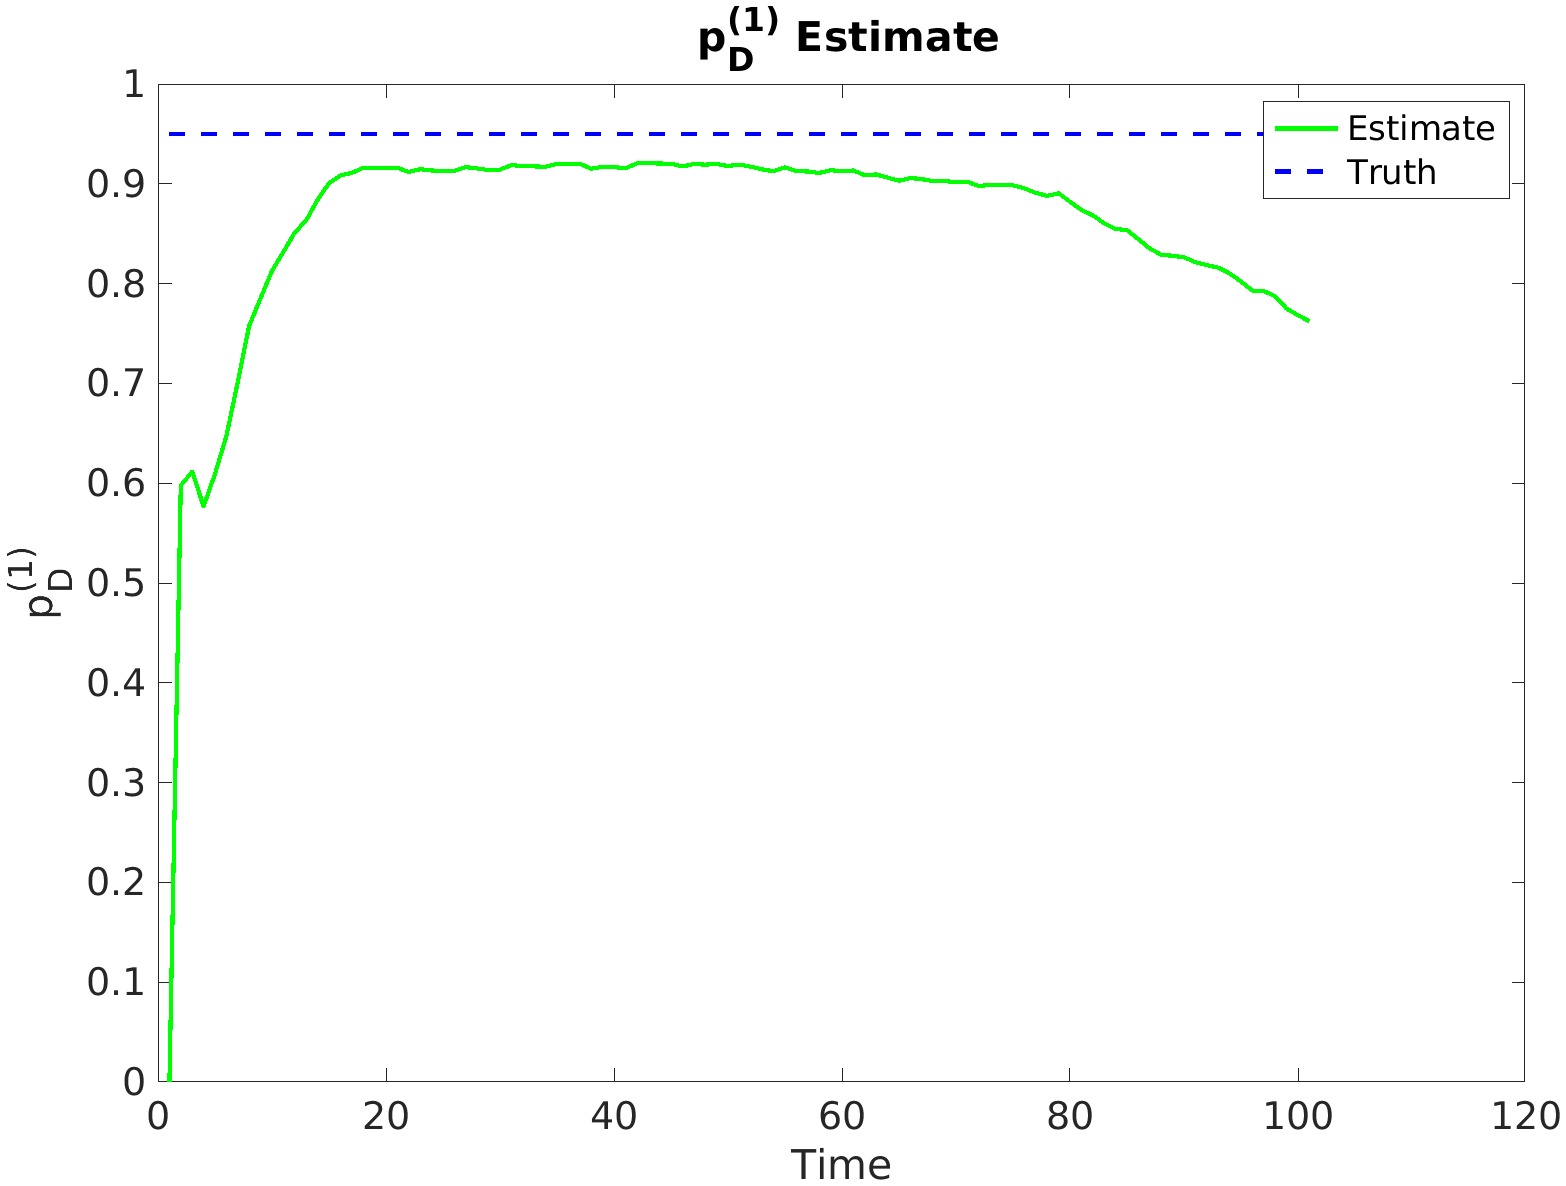
\includegraphics[width=1\linewidth]{optimal/pd1_hat.png}
    \caption{Target detection probability}
  \end{subfigure}  
  \caption{Parameter estimates from $\lambda$-$p_D$-CPHD}
  \label{fig:opt_param_est}
\end{figure}
The estimated clutter and target detection probabilities, and clutter rate from the $\lambda$-$p_D$-CPHD filter, which are also used in the adaptive LMB filter all exhibit some degree of bias, but wind up generating at least sane estimates of their respective parameters, if not extremely accurate estimates. The cardinality estimates of the adaptive LMB filter appear to be more sensitive to the errors in these parameters than those of the $\lambda$-$p_D$-CPHD filter do, with the adaptive LMB showing both a larger RMS error and a larger overall cardinality bias with the mean cardinality error. One other source of parameter estimate error is that as implemented, none of the filtering algorithms take the sensor field of view into account. When a target passes out of the field of view the intensity components associated with that target will remain, and since they stop having measurements associated with them because the target is out of the field of view they wind up skewing the parameter estimates. This can be observed easily in the estimated target detection probability. The true cardinality of visible targets starts to decrease at $t \approx 60$ as targets start to reach the edge of the field of view, and a corresponding decrease in the estimated target detection probability can be observed starting at the same time in figure \ref{fig:opt_param_est}(c).

\subsection{Parameter Effects}
Further tests were run to compare the effects of parameter choices on filter behavior. All of these filters were configured the same as in the above ``optimal'' filter tests, except as noted.
\subsubsection{Target Detection Probability ($p_D^\tgt$)}
The filters were tested with the target detection probability value passed to the filters $p_d^\tgt$ set to half of the true target detection probability.
\begin{table}[H]
  \centering
  \begin{tabular}{ c| c | c | c | c | c | c }
    & RMS $N_{err}$ & Mean $N_{err}$ & Std $N_{err}$ & Mean OSPA & Mean OSPA Loc. & Mean OSPA Card.\\
    \hline
    $GMPHD$ & 6.92 & -5.34 & 4.41 & 5.14 & 0.735 & 4.51 \\
    $\lambda-CPHD$ & 7.01 & -5.66 & 4.13 & 5.09 & 0.8 & 4.39 \\
    $\lambda-p_D-CPHD$ & 2.03 & 1.08 & 1.72 & 3.45 & 1 & 2.55 \\
    $LMB$ & 4.6 & 4.05 & 2.17 & 7.02 & 2.39 & 4.73 \\
    $Adaptive LMB$ & 2.59 & 1.84 & 1.83 & 3.88 & 1.41 & 2.56 \\
  \end{tabular}
  \caption{Filter performance with an inaccurate birth model detection probability}
  \label{tab:low_pd}
\end{table}
Changing the target detection 
\begin{figure}[H]
  \centering
  \begin{subfigure}[t]{0.49\textwidth}
    \centering
    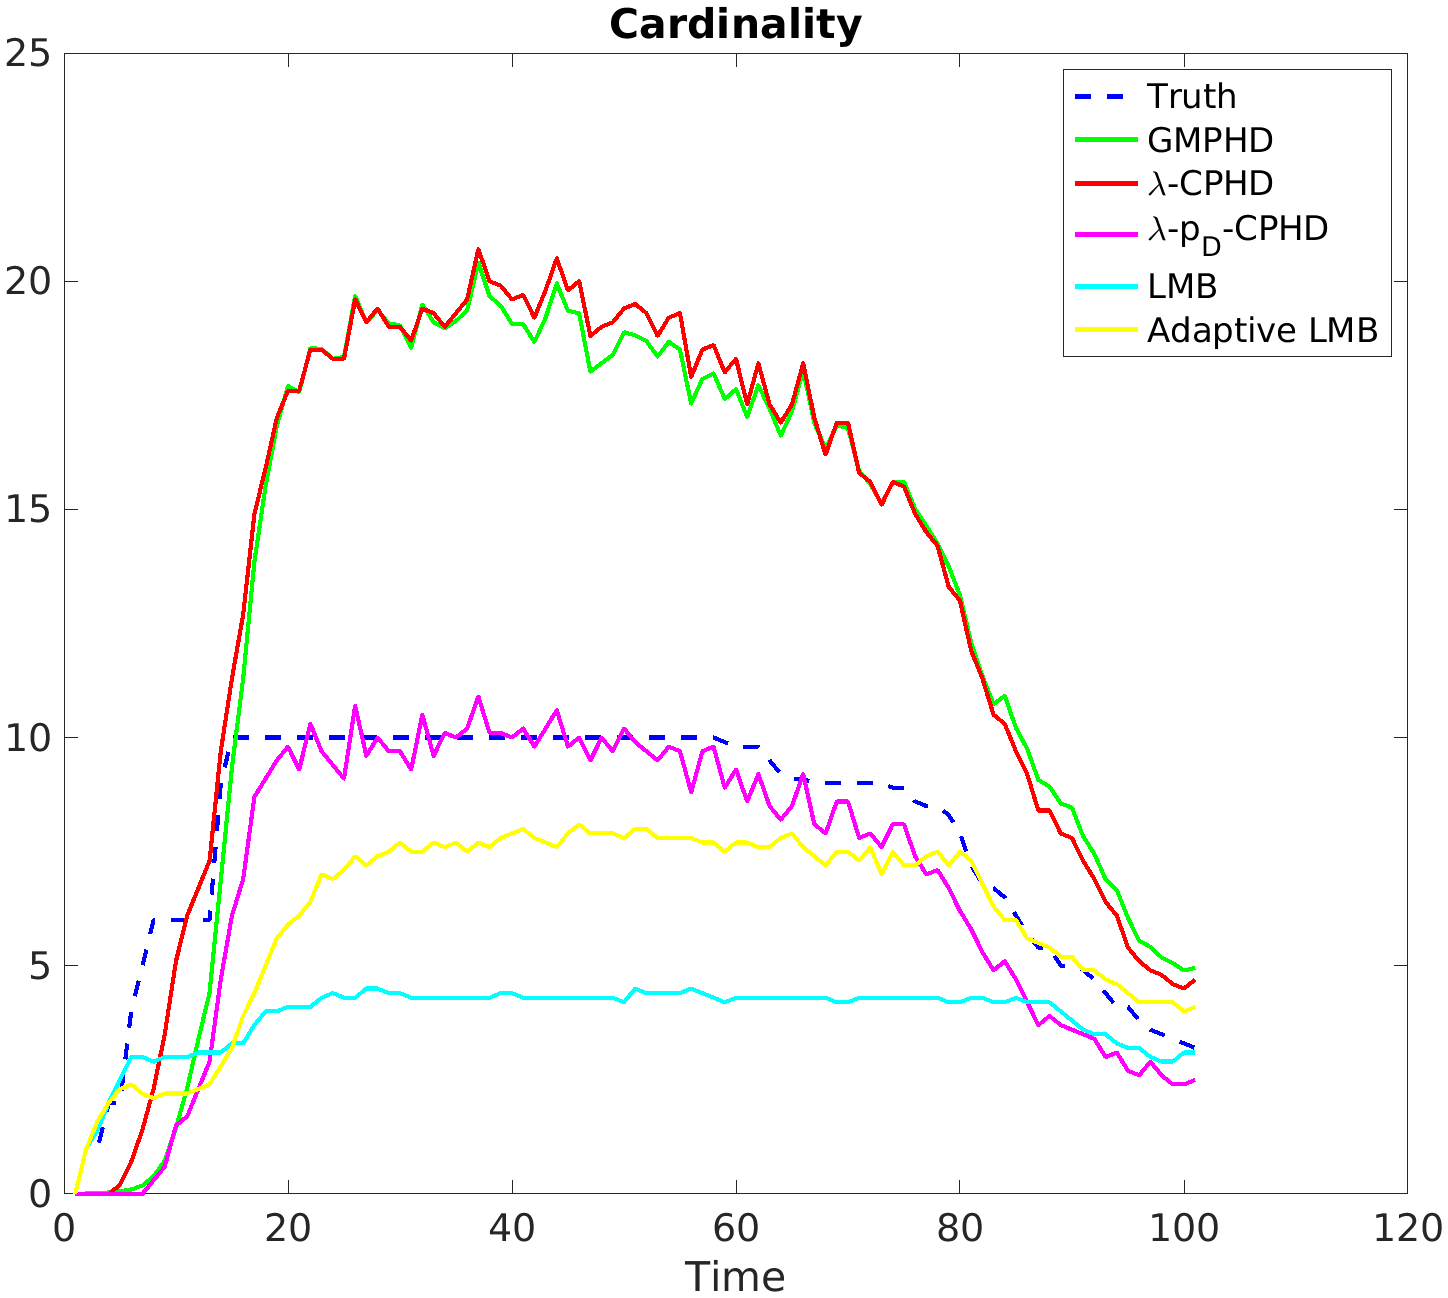
\includegraphics[width=1\linewidth]{low_pd/cardinality.png}
    \caption{Cardinality estimates}
  \end{subfigure}%
  ~ 
  \begin{subfigure}[t]{0.49\textwidth}
    \centering
    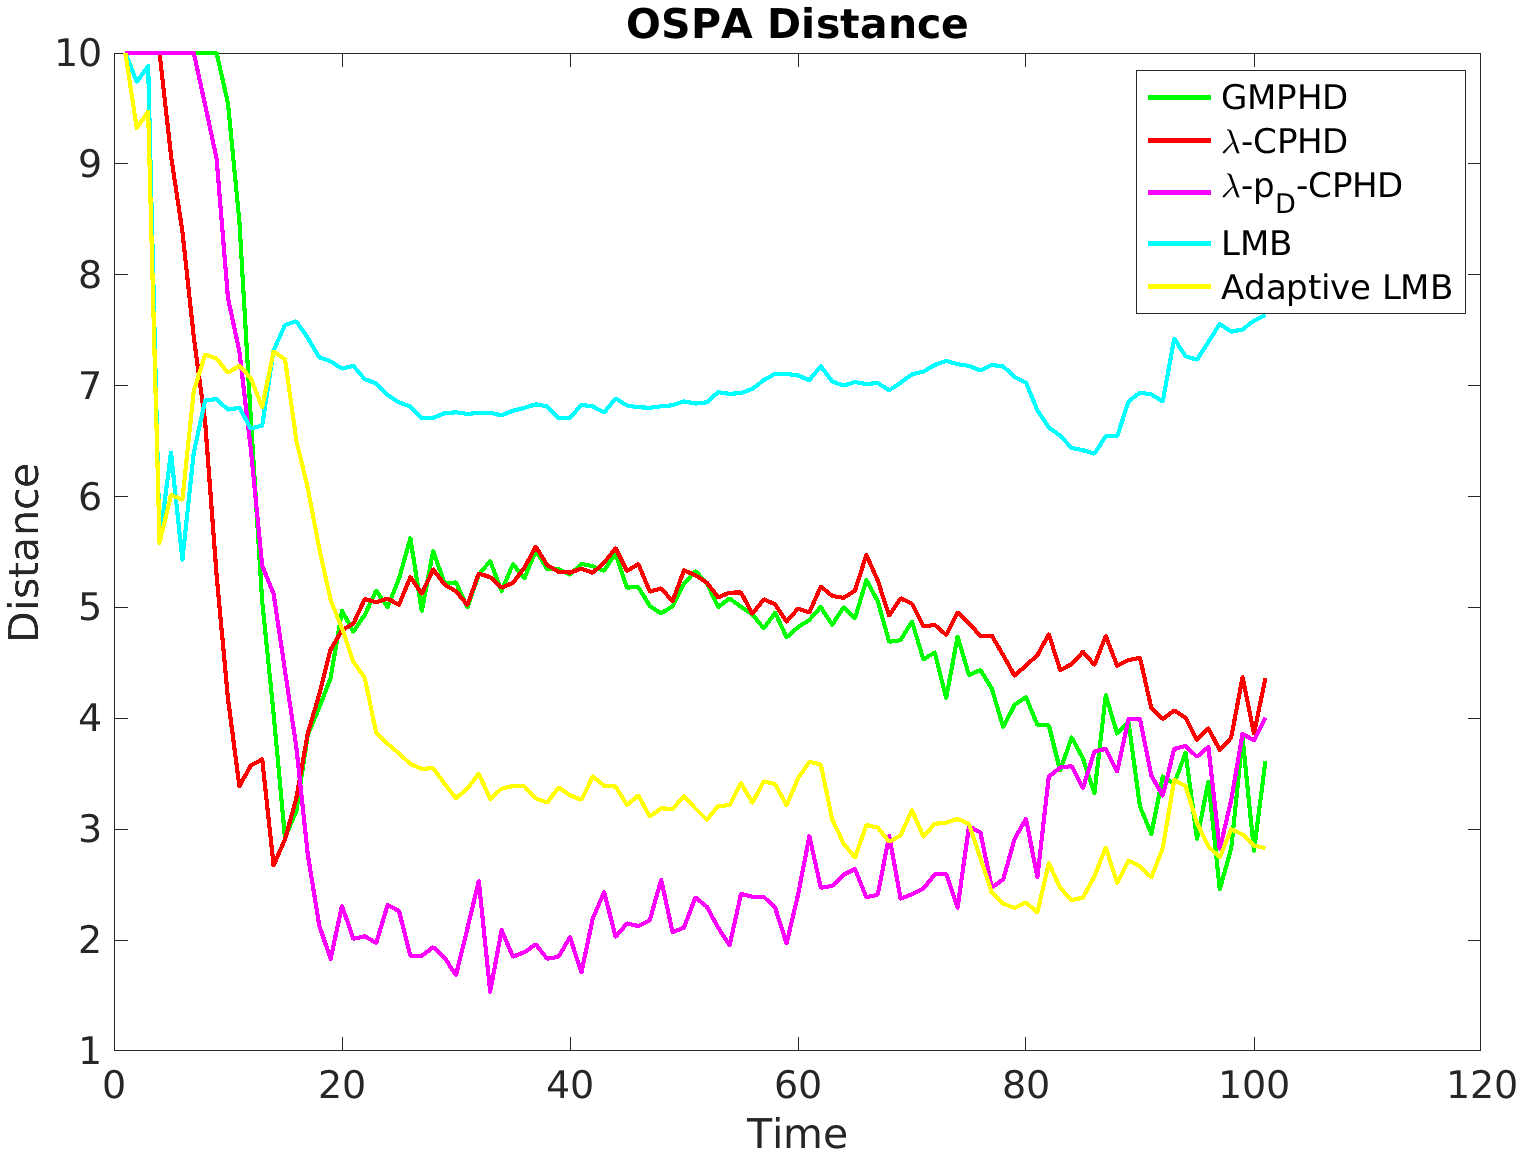
\includegraphics[width=1\linewidth]{low_pd/ospa.png}
    \caption{OSPA distances}
  \end{subfigure}
\caption{Cardinality estimates and OSPA distances for estimators with incorrect $p_D$}
\end{figure}
The GMPHD, $\lambda$-CPHD, and LMB filters all exhibit extremely high cardinality errors when run with and incorrect target detection probability. The cardinality estimates from the \lcphd and GMPHD filters both appear to be approximately twice the true cardinality. The cardinality estimate from the LMB filter on the other hand appears to be approximately half the true cardinality. The performance of the two filters that are adaptive in the target detection probability, the adaptive LMB and the \lpdcphd filter remain largely unchanged. Like in the optimal filtering case the \lpdcphd filter appears to outperform the adaptive LMB filter in terms of both cardinality and OSPA.

\subsubsection{Target Birth Model ($\Gamma^{(1)}$)}
The filters were run against a birth model consisting of a single gaussian component located along the left edge of the sensor's field of view. The weight of the component was not changed relative to the birth model used for testing the ``optimal'' filters
\begin{figure}[H]
  \centering
  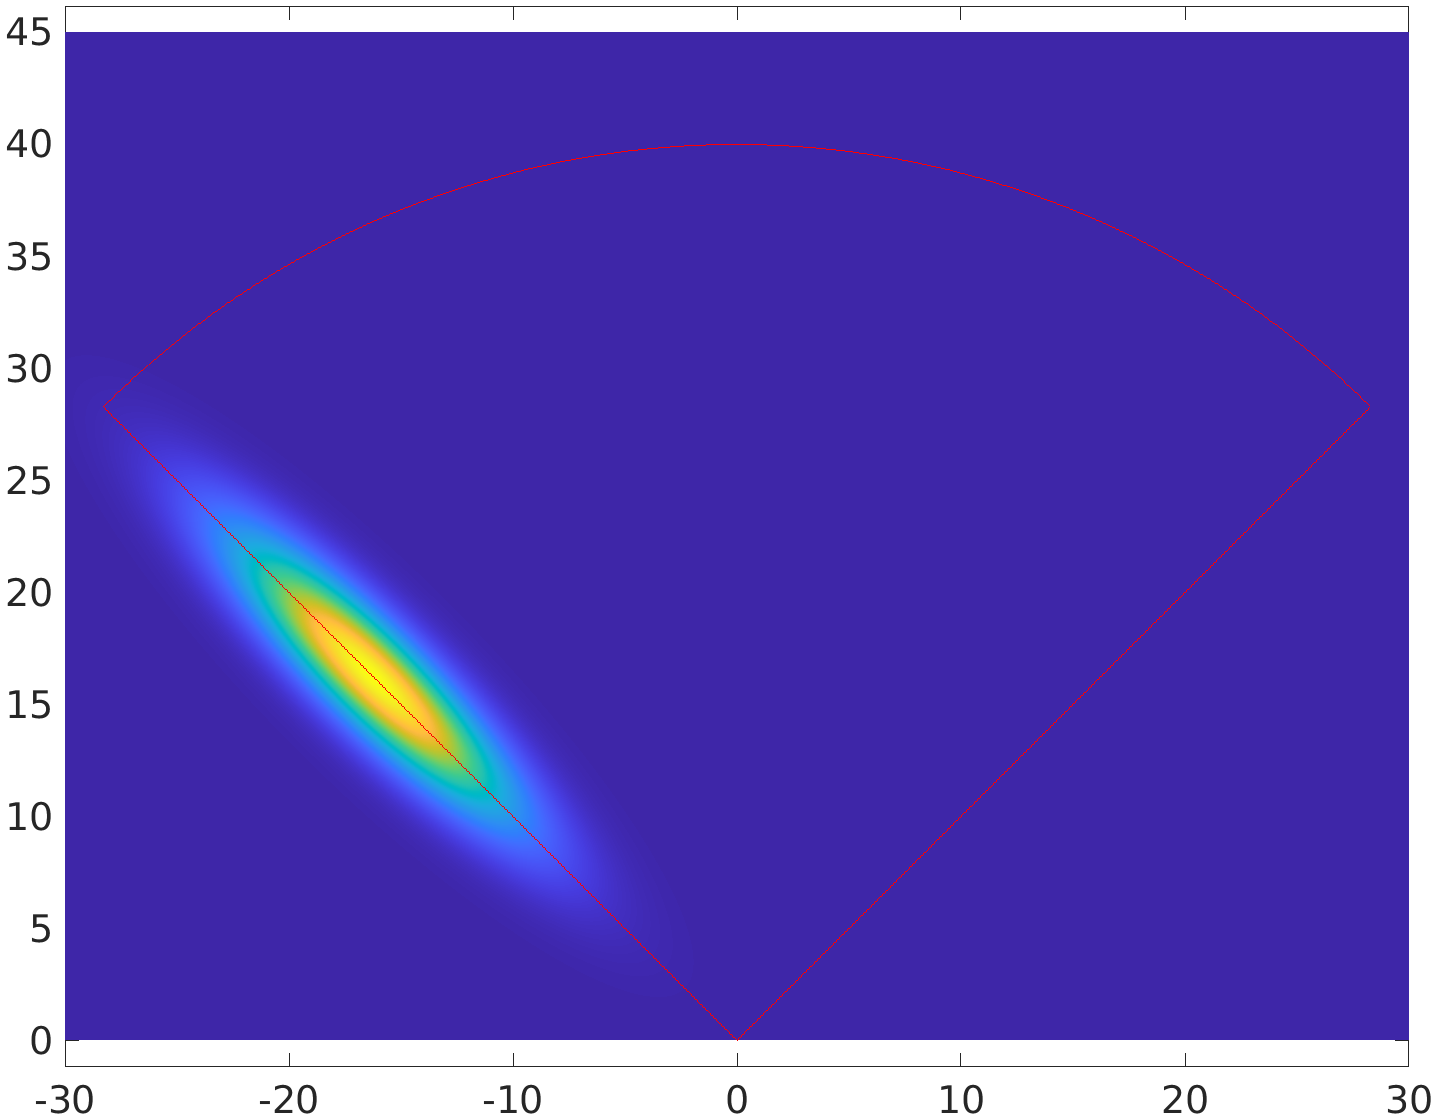
\includegraphics[width=.75\linewidth]{bad_birth/bm.png}
  \label{fig:birth_model}
  \caption{Inaccurate birth model}
\end{figure}

\begin{table}[H]
  \centering
  \begin{tabular}{ c| c | c | c | c | c | c }
    & RMS $N_{err}$ & Mean $N_{err}$ & Std $N_{err}$ & Mean OSPA & Mean OSPA Loc. & Mean OSPA Card.\\
    \hline
    $GMPHD$ & 2.63 & 0.587 & 2.57 & 3.72 & 0.784 & 3.04 \\
    $\lambda-CPHD$ & 2.38 & 0.166 & 2.38 & 3.42 & 1.06 & 2.46 \\
    $\lambda-p_D-CPHD$ & 3.95 & 2.59 & 2.98 & 4.61 & 0.804 & 3.9 \\
    $LMB$ & 5.17 & 4.65 & 2.25 & 6.73 & 1.12 & 5.72 \\
    $Adaptive LMB$ & 6.36 & 5.63 & 2.96 & 7.9 & 1.57 & 6.43 \\
  \end{tabular}
  \caption{Filter performance with an inaccurate birth model}
  \label{tab:}
\end{table}
\begin{figure}[H]
  \centering
  \begin{subfigure}[t]{0.49\textwidth}
    \centering
    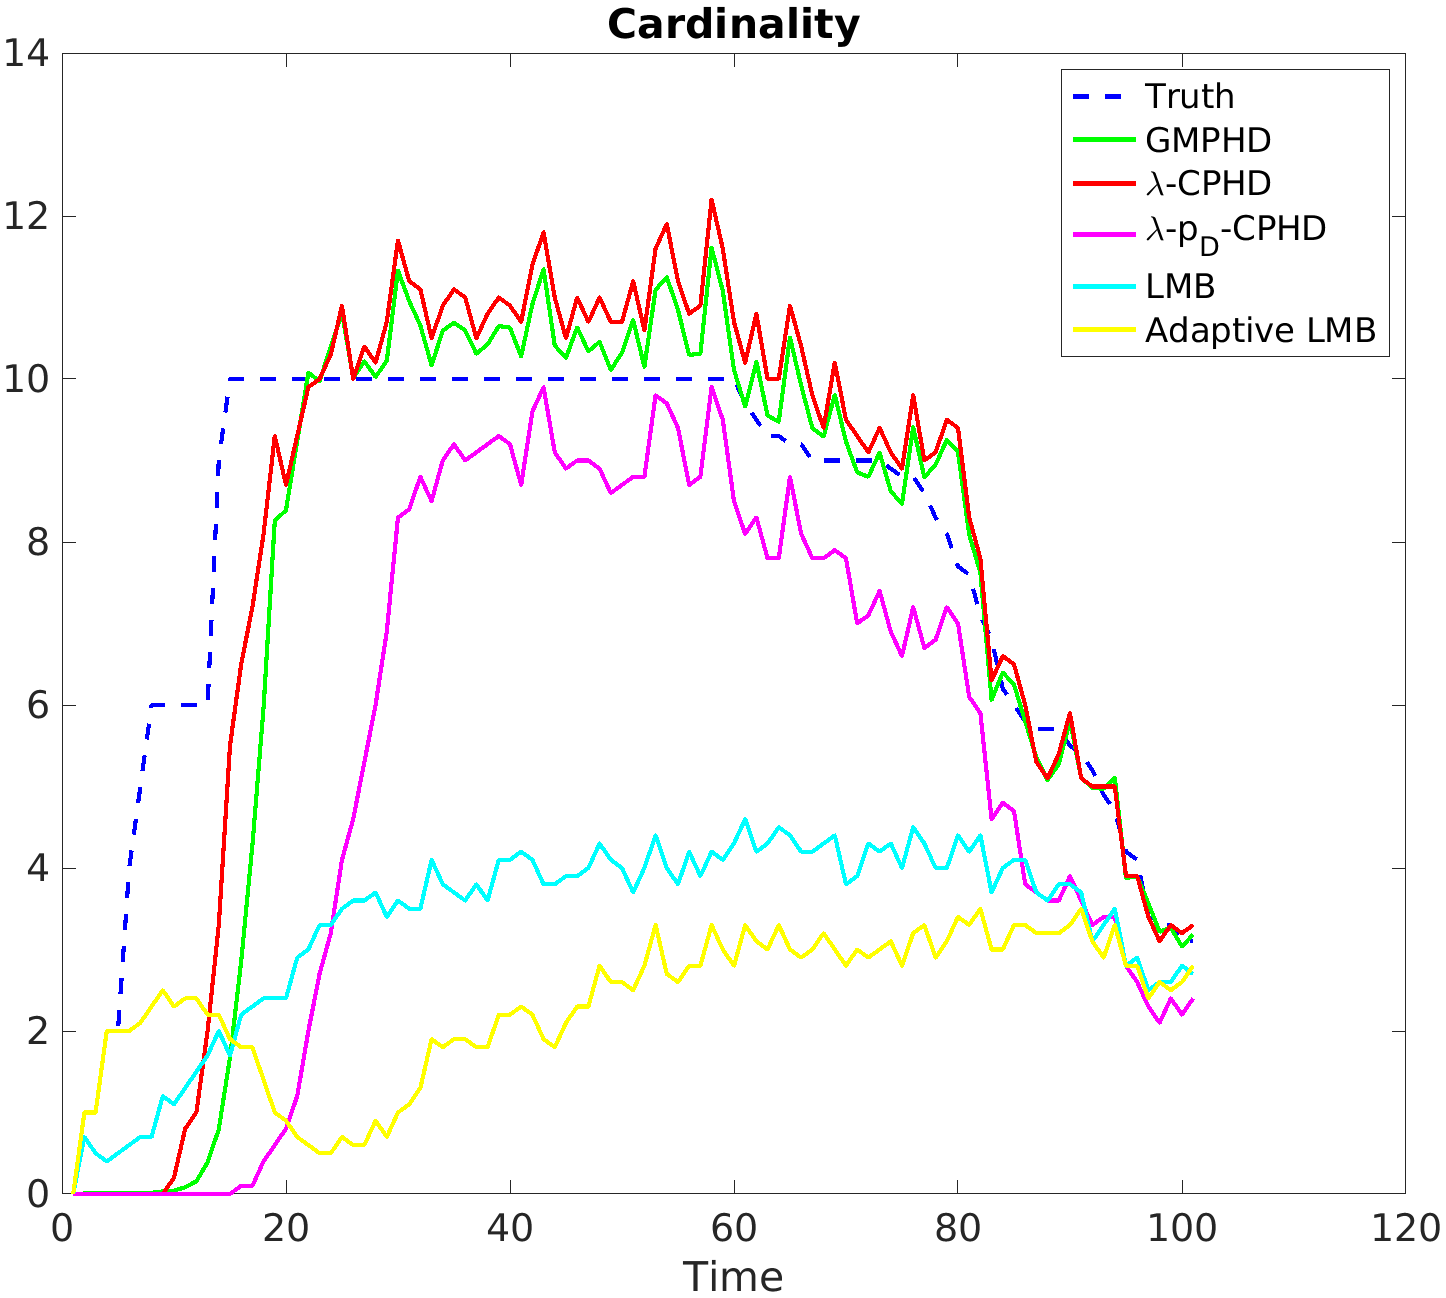
\includegraphics[width=1\linewidth]{bad_birth/cardinality.png}
    \caption{Cardinality estimates}
  \end{subfigure}%
  ~ 
  \begin{subfigure}[t]{0.49\textwidth}
    \centering
    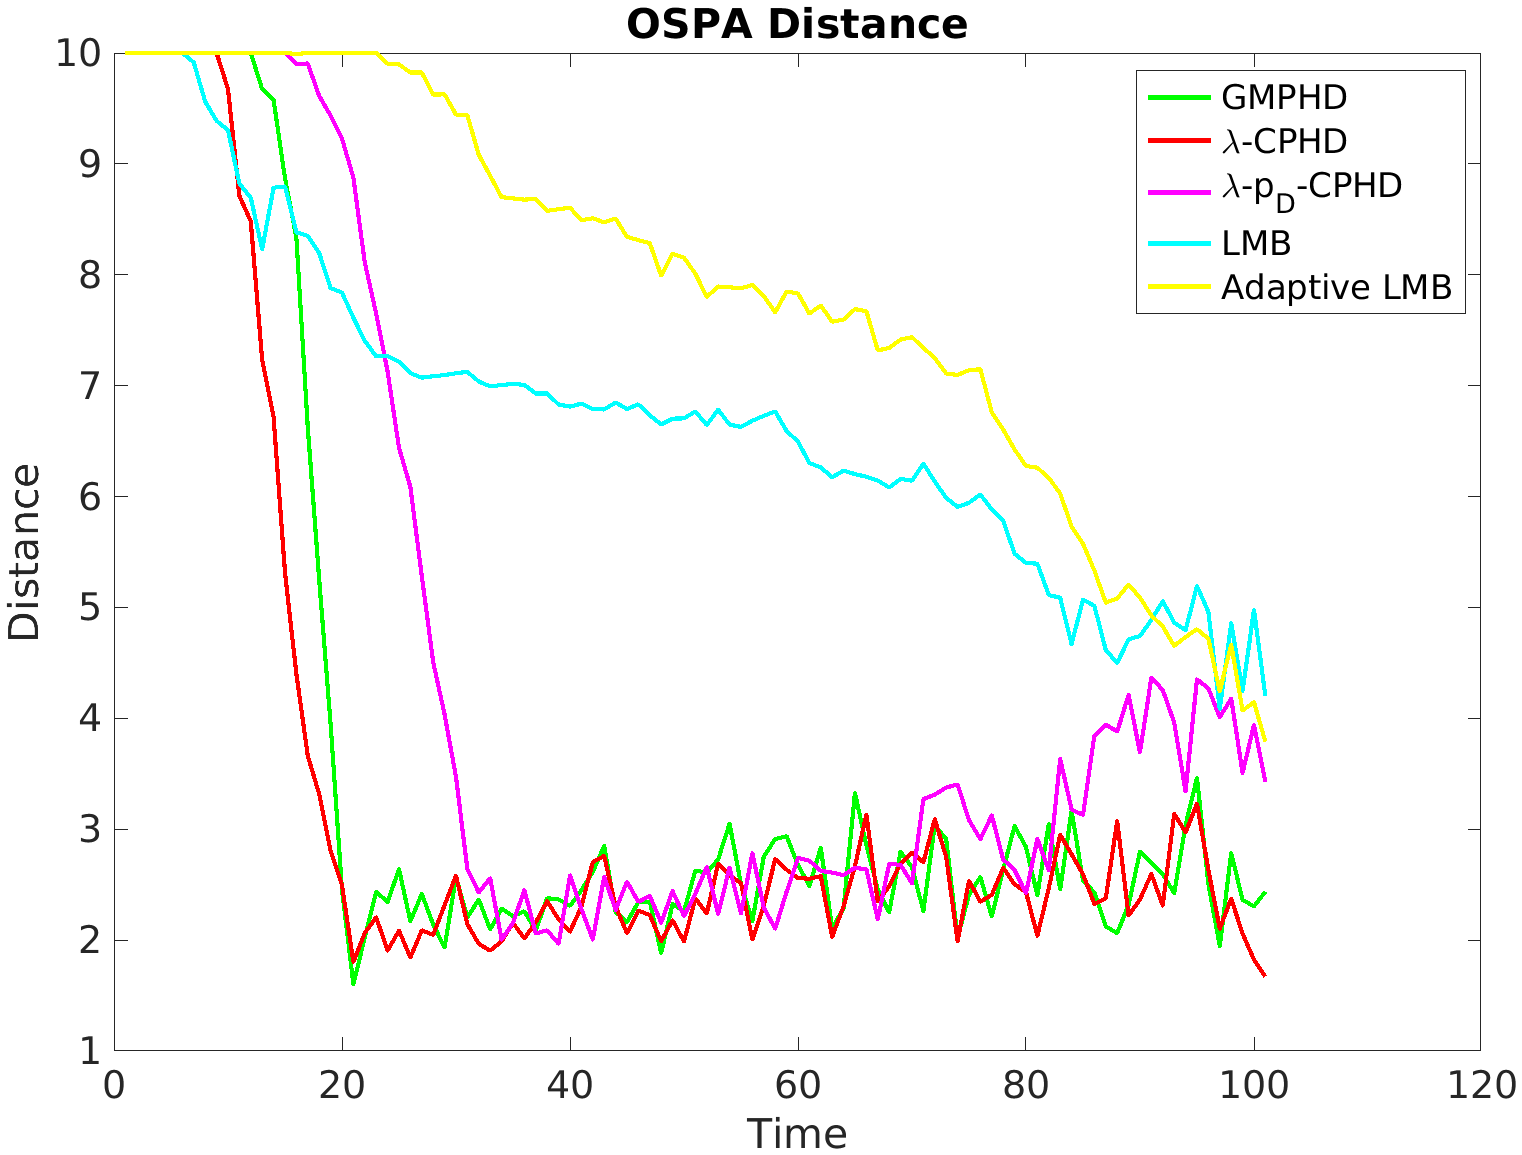
\includegraphics[width=1\linewidth]{bad_birth/ospa.png}
    \caption{OSPA distances}
  \end{subfigure}
  \caption{Cardinality estimates and OSPA distances for estimators with incorrect target birth model}
  \label{fig:bad_bm_performance}
\end{figure}
The GMPHD, $\lambda$-CPHD, and $\lambda$-$p_D$-CPHD filters all seem to be much more robust to errors in the birth model than the LMB and adaptive LMB filters. While all of the filters show an increased OSPA distance relative to their optimal results, the OSPA distances for for the LMB and adaptive LMB filters more than doubled. This inaccuracy seems to be driven primarily by cardinality error. As shown in figure \ref{fig:bad_bm_performance}(a) both of these filters consistently tracked fewer than half of the targets.
\subsubsection{Target Survival Probability ($p_S^{(1)}$)}
The target survival probability value, $p_S^\tgt$, that was passed to the filters was increased from the ``true'' value of $0.9$ to $0.99$ for the next test.
\begin{table}[H]
  \centering
\begin{tabular}{ c| c | c | c | c | c | c }
   & RMS $N_{err}$ & Mean $N_{err}$ & Std $N_{err}$ & Mean OSPA & Mean OSPA Loc. & Mean OSPA Card.\\
\hline
  $GMPHD$ & 1.91 & -0.68 & 1.79 & 3.34 & 0.853 & 2.59 \\
  $\lambda-CPHD$ & 2.01 & -1.09 & 1.69 & 3.01 & 1.27 & 1.84 \\
  $\lambda-p_D-CPHD$ & 2.87 & -1.41 & 2.5 & 3.81 & 0.936 & 2.98 \\
  $LMB$ & 1.64 & -1.14 & 1.18 & 2.51 & 0.998 & 1.61 \\
  $Adaptive LMB$ & 3.3 & -0.64 & 3.24 & 3.59 & 1.37 & 2.32 \\
\end{tabular}
  \caption{Filter performance with an inaccurate survival probability}
  \label{tab:high_ps}
\end{table}
The primary effect of running the filters with a target survival probability of $0.99$ seemed to be to add a small bias to most of the cardinality estimates. The exception is the adaptive LMB filter, whose cardinality estimate appears to start to diverge once the visible target population starts to decrease. One possible reason for this is that the estimated target detection probability also appears to be diverging as seen in Figure \ref{fig:high_ps_param_est}(c).

\begin{figure}[H]
  \centering
  \begin{subfigure}[t]{0.49\textwidth}
    \centering
    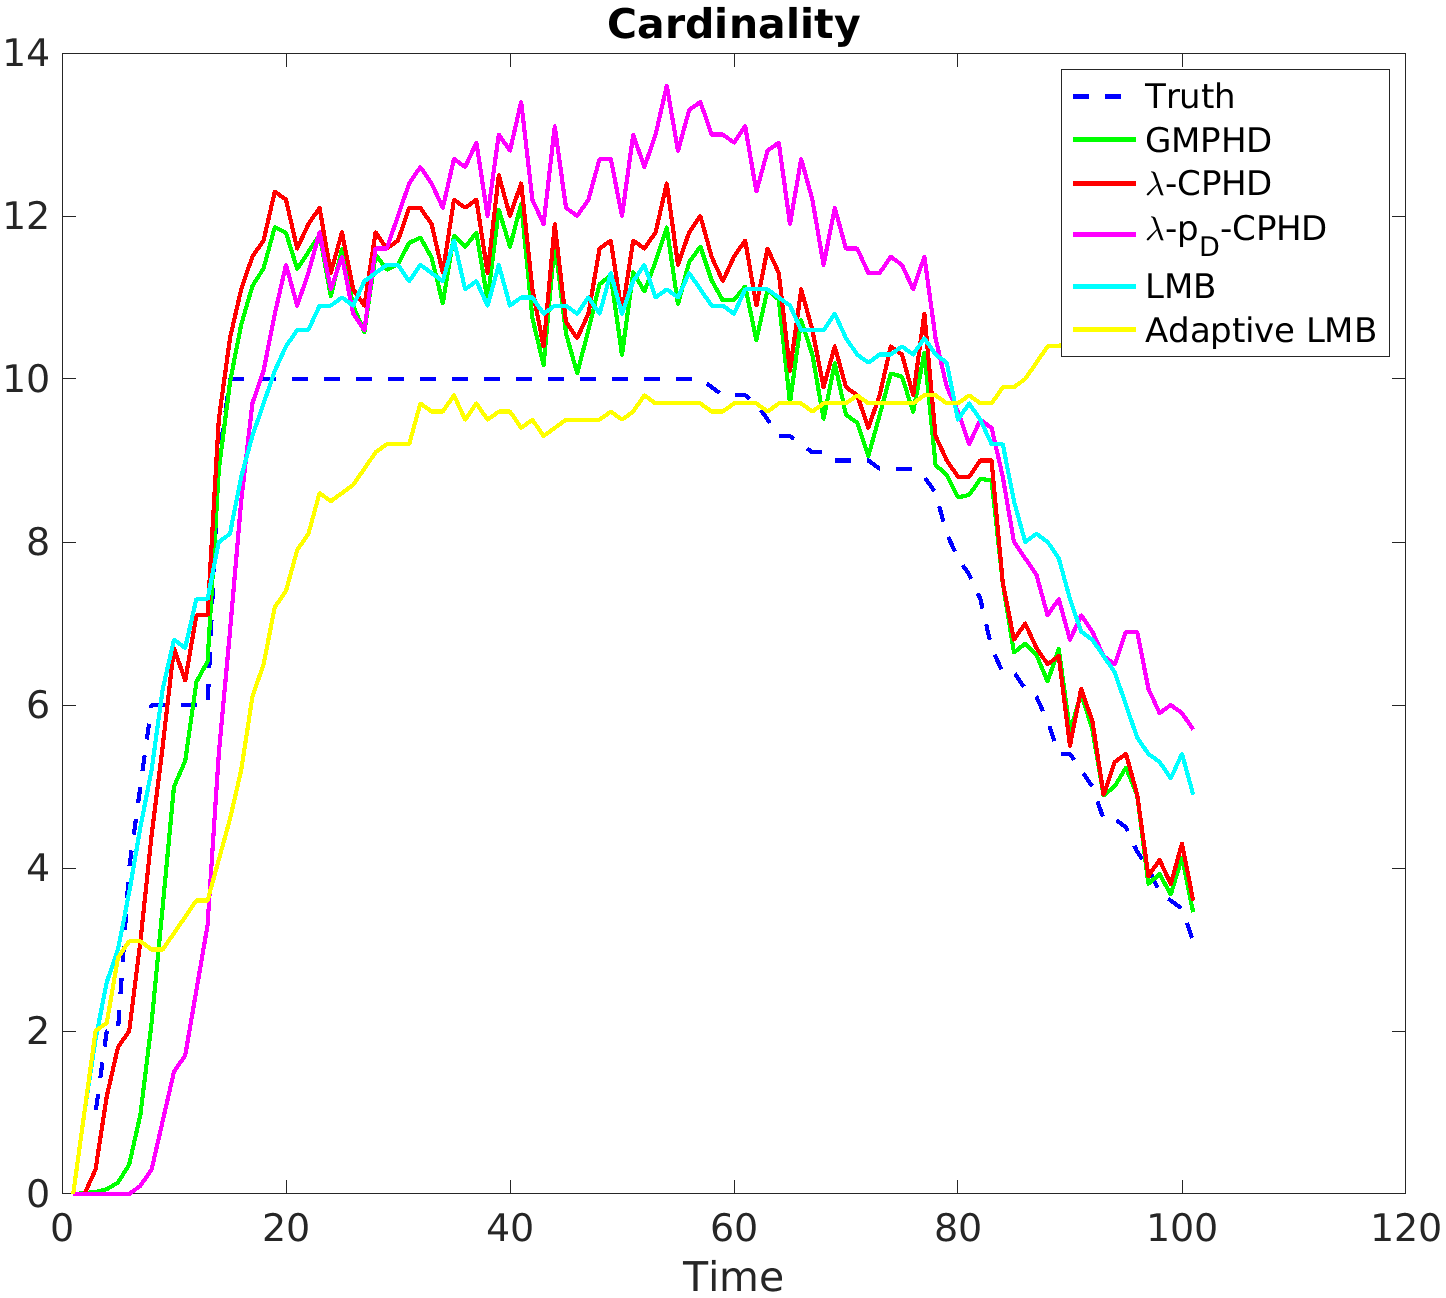
\includegraphics[width=1\linewidth]{high_ps/cardinality.png}
    \caption{Cardinality estimates}
  \end{subfigure}%
  ~ 
  \begin{subfigure}[t]{0.49\textwidth}
    \centering
    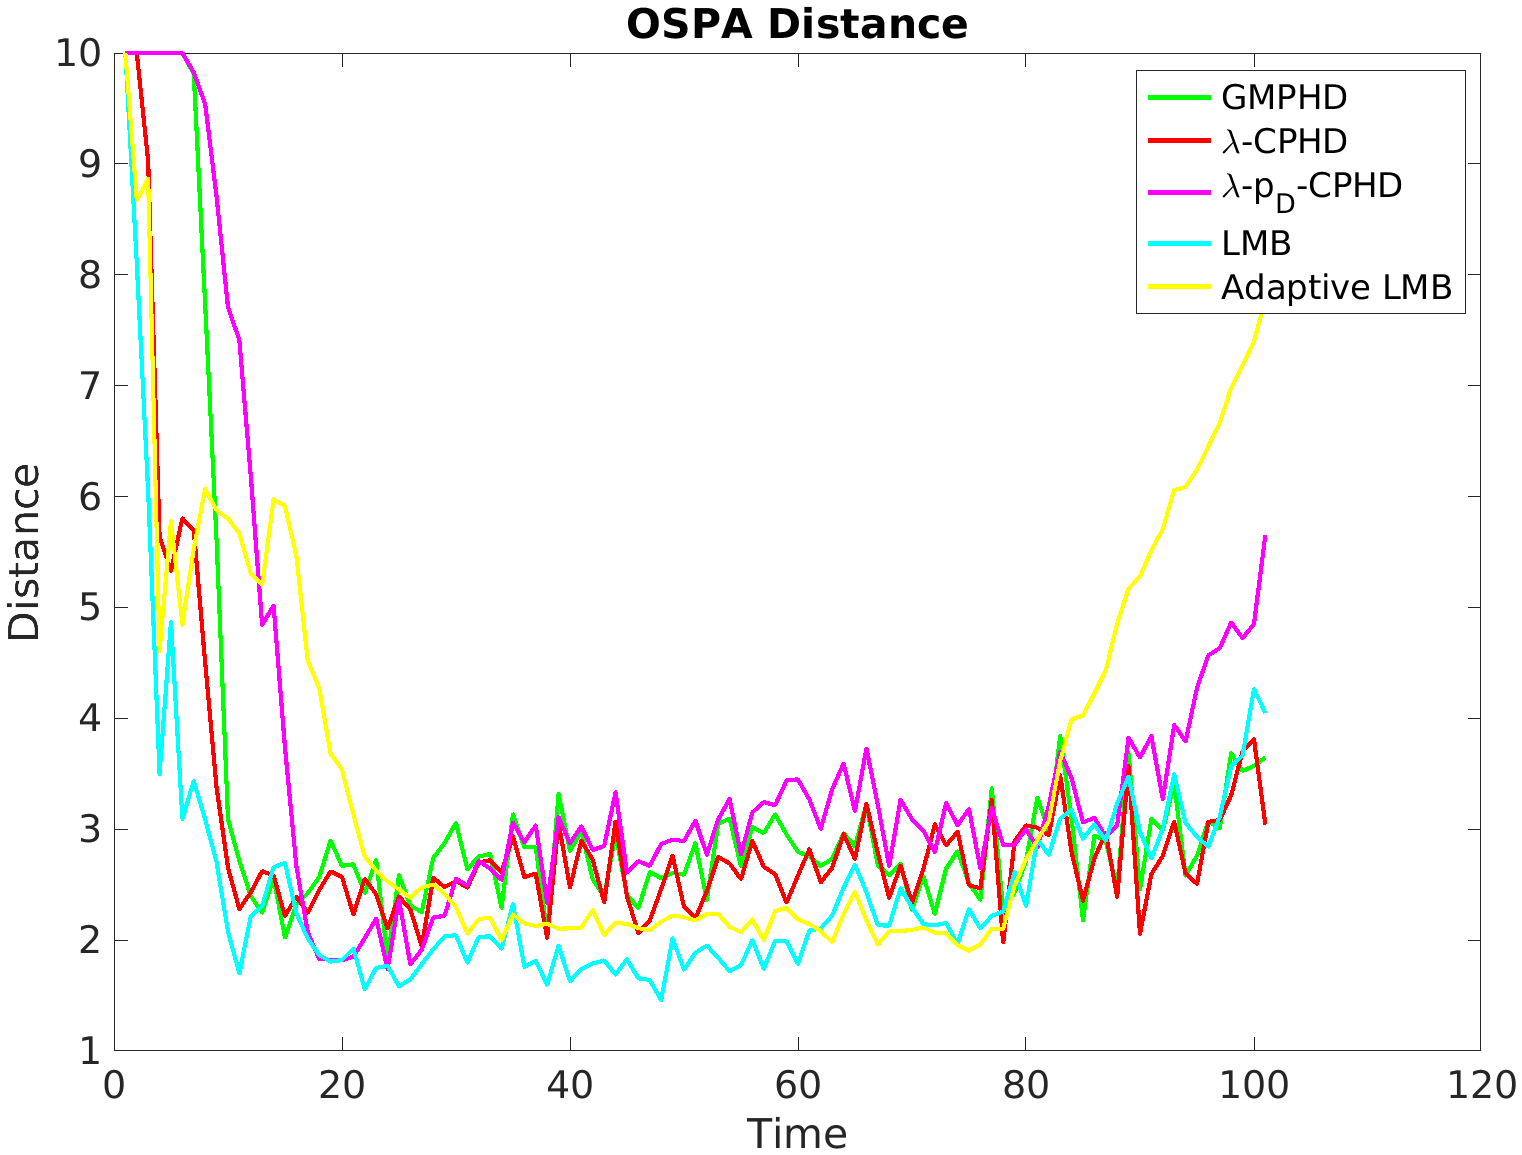
\includegraphics[width=1\linewidth]{high_ps/ospa.png}
    \caption{OSPA distances}
  \end{subfigure}
\caption{Cardinality estimates and OSPA distances for estimators with incorrect target survival probability}
\end{figure}
\begin{figure}[H]
  \centering
  \begin{subfigure}[t]{0.32\textwidth}
    \centering
    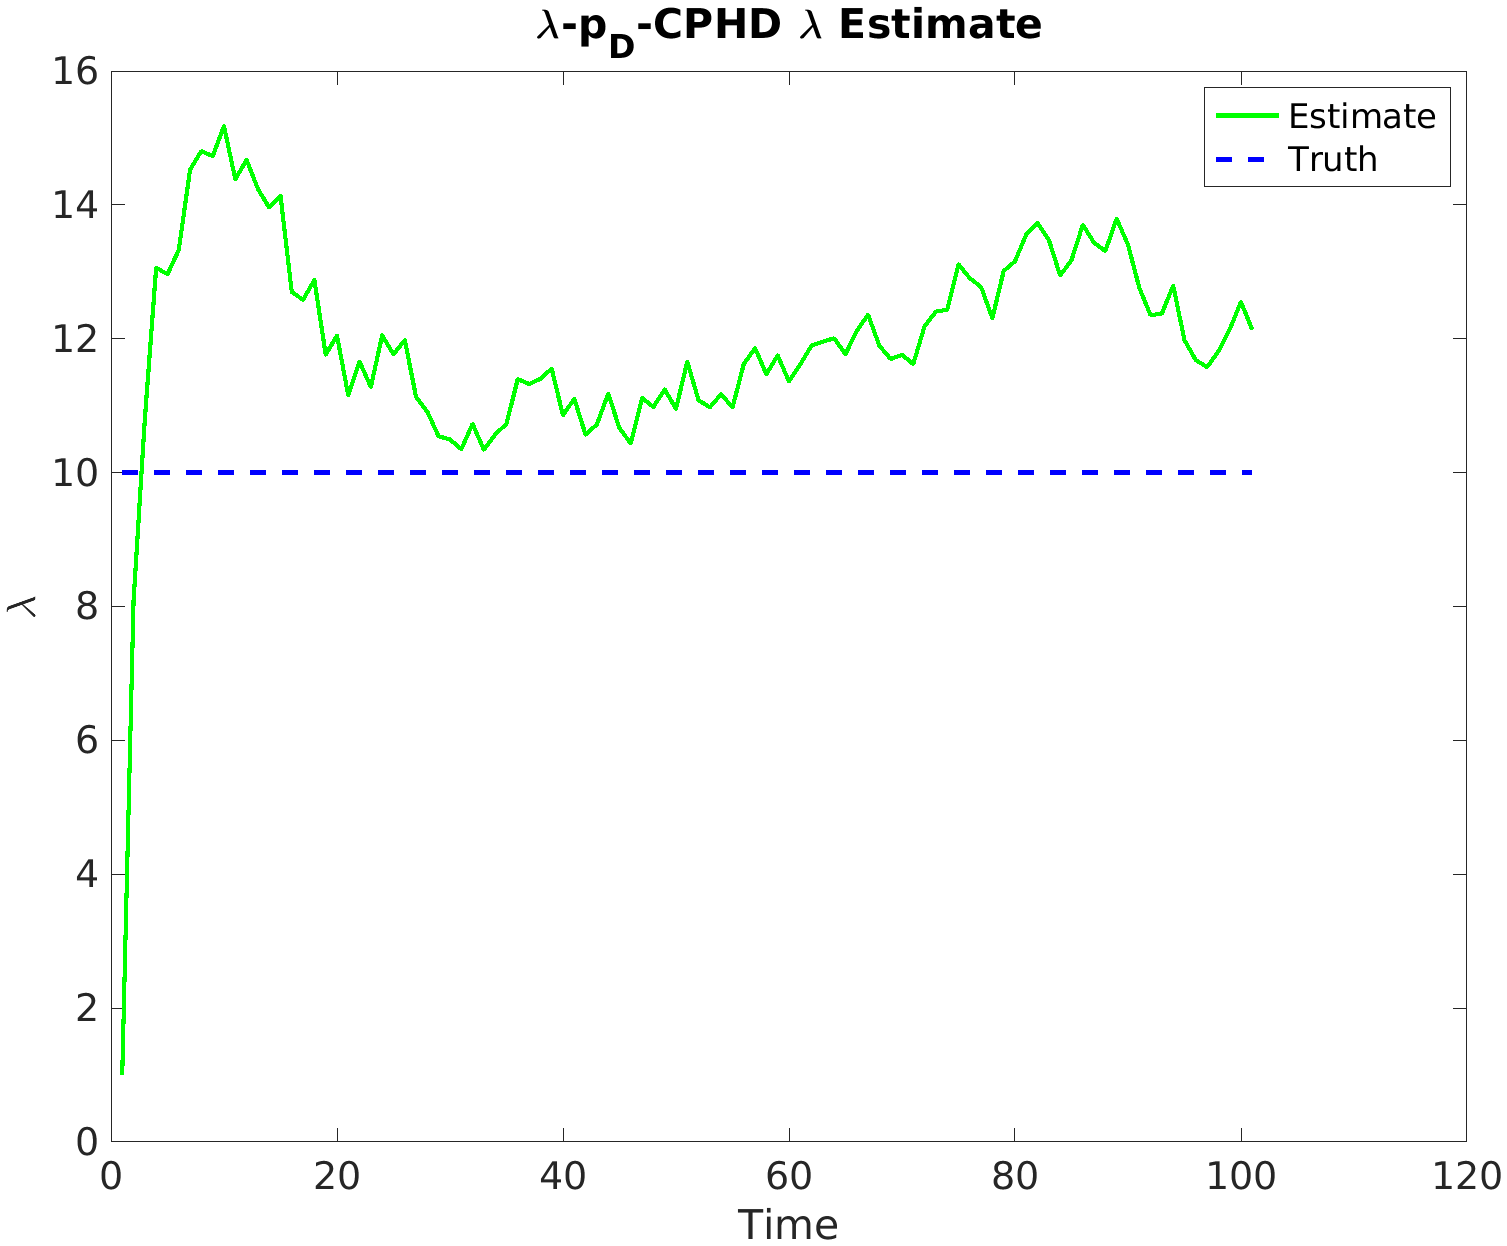
\includegraphics[width=1\linewidth]{high_ps/lpdcphd_lambda_hat.png}
    \caption{Clutter rate}
  \end{subfigure}%
  ~ 
  \begin{subfigure}[t]{0.32\textwidth}
    \centering
    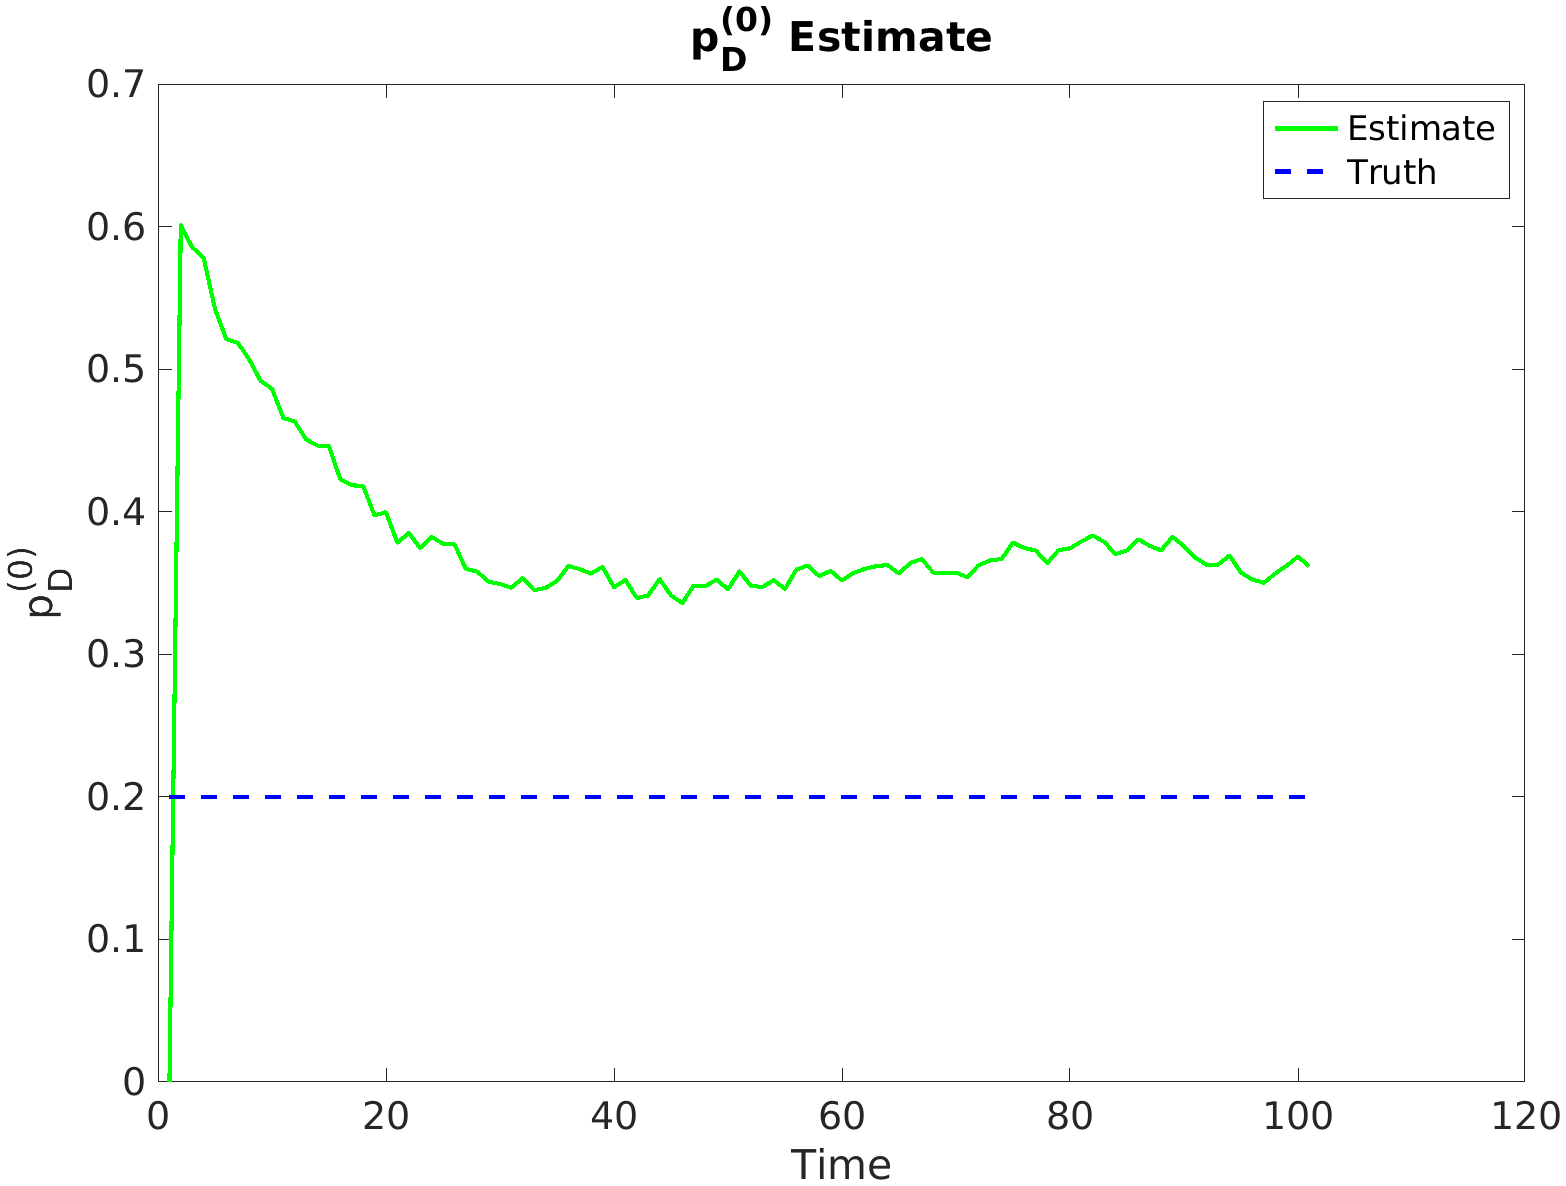
\includegraphics[width=1\linewidth]{high_ps/pd0_hat.png}
    \caption{Clutter detection probability}
  \end{subfigure}
  ~ 
  \begin{subfigure}[t]{0.32\textwidth}
    \centering
    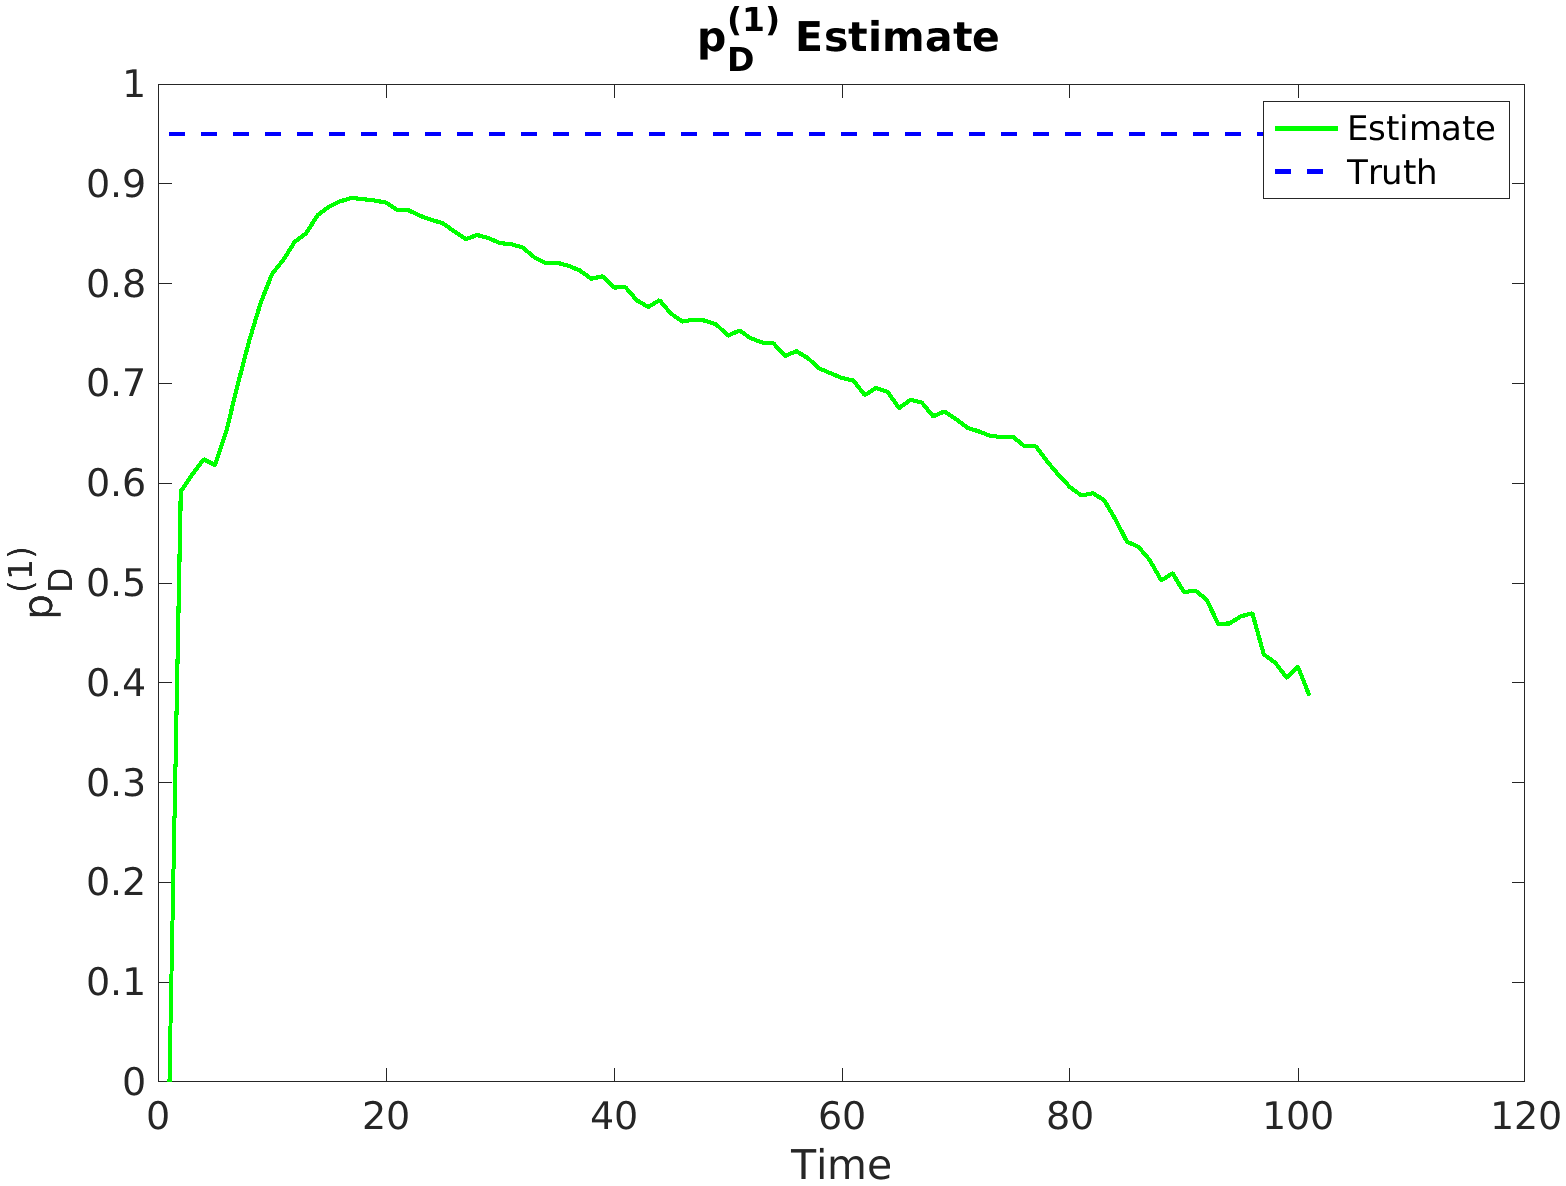
\includegraphics[width=1\linewidth]{high_ps/pd1_hat.png}
    \caption{Target detection probability}
  \end{subfigure}  
  \caption{Parameter estimates from $\lambda$-$p_D$-CPHD with incorrect target survival probability}
  \label{fig:high_ps_param_est}
\end{figure}

\subsubsection{Clutter Rate ($\lambda$)}
Finally, a test was run with the clutter rate for each filter set to half of the actual clutter rate.
\begin{table}[H]
  \centering
  \begin{tabular}{ c| c | c | c | c | c | c }
    & RMS $N_{err}$ & Mean $N_{err}$ & Std $N_{err}$ & Mean OSPA & Mean OSPA Loc. & Mean OSPA Card.\\
    \hline
    $GMPHD$ & 3.32 & -2.61 & 2.06 & 3.84 & 0.755 & 3.19 \\
    $\lambda-CPHD$ & 1.64 & -0.565 & 1.54 & 2.79 & 1.22 & 1.66 \\
    $\lambda-p_D-CPHD$ & 2.06 & 1.1 & 1.75 & 3.38 & 0.956 & 2.53 \\
    $LMB$ & 2.26 & -1.89 & 1.23 & 3.04 & 1.04 & 2.1 \\
  $Adaptive LMB$ & 2.34 & 1.43 & 1.85 & 3.51 & 1.4 & 2.21 \\
\end{tabular}  
  \caption{Filter performance with an inaccurate clutter rate}
  \label{tab:low_clutter}
\end{table}
\begin{figure}[H]
  \centering
  \begin{subfigure}[t]{0.49\textwidth}
    \centering
    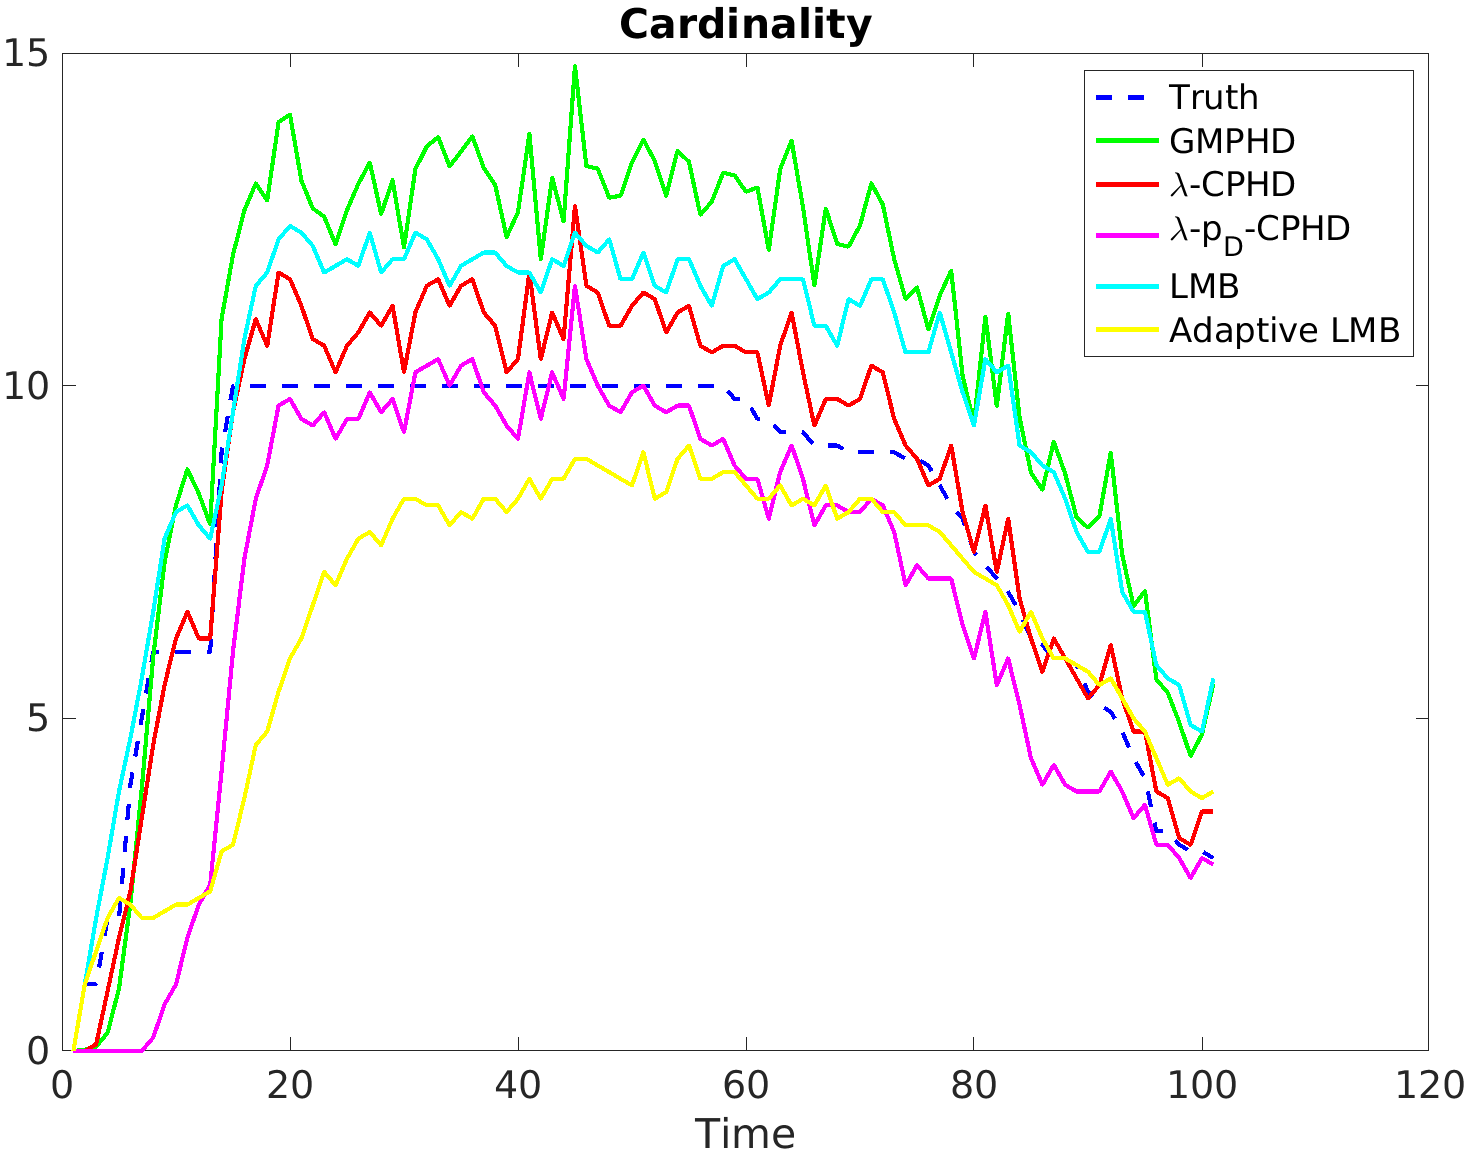
\includegraphics[width=1\linewidth]{low_clutter/cardinality.png}
    \caption{Cardinality estimates}
  \end{subfigure}%
  ~ 
  \begin{subfigure}[t]{0.49\textwidth}
    \centering
    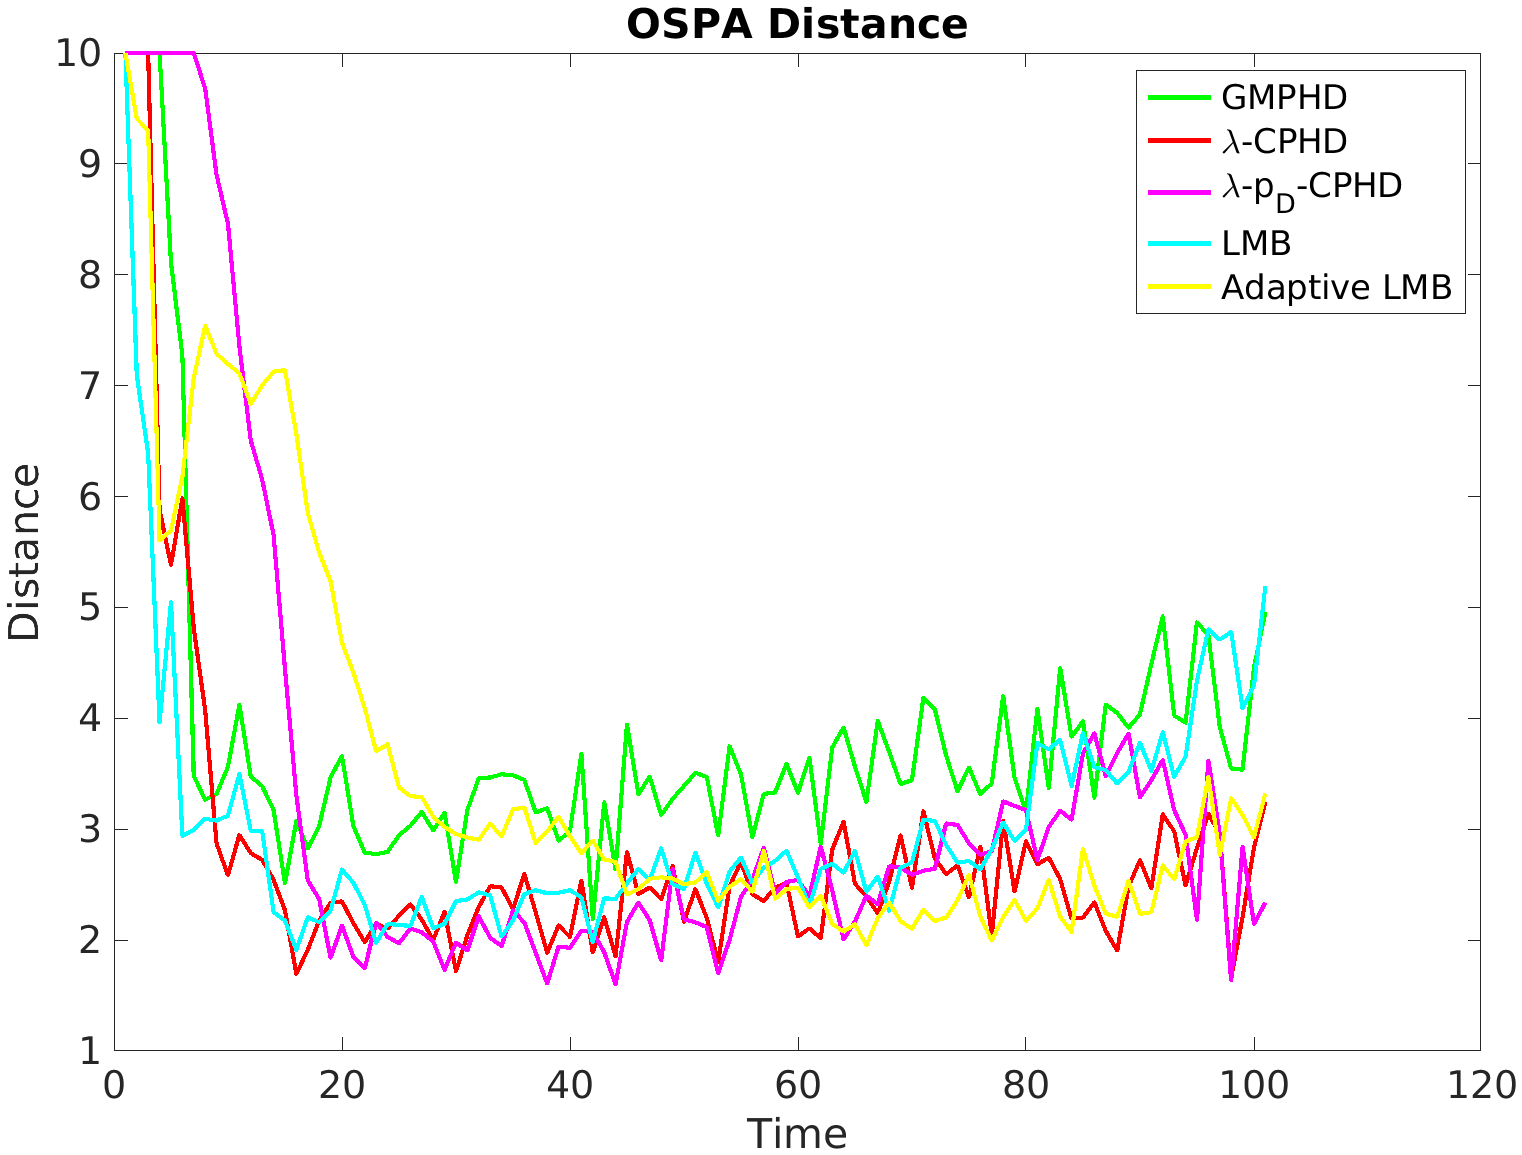
\includegraphics[width=1\linewidth]{low_clutter/ospa.png}
    \caption{OSPA distances}
  \end{subfigure}
\caption{Cardinality estimates and OSPA distances for estimators with incorrect clutter rate}
\end{figure}
The \lcphd, \lpdcphd, and adaptive LMB filter all estimate their own clutter rates, and so were unaffected by the incorrect clutter rate. The LMB filter still performed reasonably well, but not as well as the \lpdcphd did. The GMPHD filter appeared to be very susceptible to cardinality errors caused by the incorrect clutter rate and exibited a significant bias in the cardinality of its estimates.

\section{Conclusions}
Under optimal conditions the labeled multi-Bernoulli filter clearly outperformed all of the other filters, with the lowest OSPA score and almost 0 cardinality bias; however, it appears to be very sensitive to differences between the model parameters it uses and the true system. This was especially true for the target detection probability and birth model, where inaccuracies in the parameters resulted in significant estimation errors. The \lcphd and GMPHD were similarly extremely susceptible to errors in the target detection probability, which induced significant biases in the cardinality estimates. The \lpdcphd and the adaptive LMB filter were unsurprisingly the most robust to incorrect parameters, as they have the ability to estimate some of the parameters on the fly. However, the adaptive LMB filter did appear to have a strange sensitivity to survival probability that none of the other filters exhibited. The \lpdcphd filter was almost never the best performing filter in any of the tests; however, it appeared to be robust to almost all of the modelling errors that were tested. In a situation that can be well modeled a filter like the LMB will almost certainly outperform the \lpdcphd. However, in real world tracking applications, where the true model parameters are often not well known the more robust \lpdcphd filter seems like a better choice. Additionally, in many  real world applications being able to provide better ``worst case'' performance can be more important than best case performance, and the ``worst case'' performance of the \lpdcphd filter was significantly better than any of the other 4 filters that were tested. The main drawback of the \lpdcphd filter compared to the adaptive LMB filter is that the \lpdcphd filter does not provide track labels. For applications that require labels the adaptive LMB filter appears to represent the best tradeoff between robustness and performance.\\
\\
Another reason that the \lpdcphd filter is an attractive choice is that it offers a good balance of performance and computational complexity. The execution times for each filter were tracked during the testing, and the average time per estimate was calculated for each filter

\begin{table}[H]
  \centering
  \begin{tabular}{ c| c }
    & Mean Est. Time (s) \\
      \hline
      $GMPHD$ & 0.03 \\
    $\lambda-CPHD$ & 0.06 \\
    $\lambda-p_D-CPHD$ & 0.07 \\
    $LMB$ & .23 \\
    $Adaptive LMB$ & .30 \\
  \end{tabular}
  \caption{Average estimation time}
  \label{tab:exec_time}
\end{table}
and while none of these implementations were done with a significant emphasis on performance, these numbers give a good ``order of magnitude'' comparison of the computational requirements for each filter.


% Bibliography
\clearpage
\pagebreak
\printbibliography


\end{document}
